\documentclass[11pt,a4paper,titlepage]{article}
\usepackage[utf8]{inputenc}
\usepackage[english]{babel}
\usepackage{amsmath}
\usepackage{amsfonts}
\usepackage{amssymb}
\usepackage[left=2cm,right=2cm,top=2cm,bottom=2cm]{geometry}
\usepackage{hyperref}
\usepackage{graphicx}
\usepackage[labelfont=bf]{caption}
\usepackage{subcaption}
\usepackage{asymptote}
\usepackage[space]{grffile}

\author{Adrian Wälchli}
\title{Bachelor Project Journal}

\begin{document}

\maketitle
\begin{abstract}
This report presents an overview of my bachelor thesis. We discuss several approaches to problems, experiments, ideas and evaluate results. This document will be extended over time as the project evolves.
\end{abstract}

\tableofcontents
\newpage

\section{Related work}
The basis of this project are the papers from \cite{WETZ_TOMO, WETZ_TENS}. Additional papers used for the work are: Light Field Rendering by Marc Levoy and Pat Hanrahan, Fourier Slice Photography by Ren Ng, Light Field Photography with a Hand-held Plenoptic Camera by Ren Ng et al. 

\section{Types of light fields} \label{sec:lftypes}
In this project, I encountered two types of 4D light fields that are captured using camera grids. The most common way of acquiring a light field is to capture a scene with a 2D-grid of cameras where the optical axes of the cameras are orthogonal to the camera grid. Since the look-at-point of each camera is different, this setup will result in a shift in the images formed on the sensors. An alternative way to capture the scene is to fix the look-at-point for every camera, preferably at the origin of the  scene. This is the type of light fields primarily used in the paper from \cite{WETZ_TOMO}. 
\\
In addition, the images can be optained using either perspective or orthographic projections. Sheared projections can also be used as mentioned in \cite[p.~4]{LEVO_LFREN}.

\begin{figure}
	\centering
	\begin{subfigure}[b]{0.4\textwidth}
 		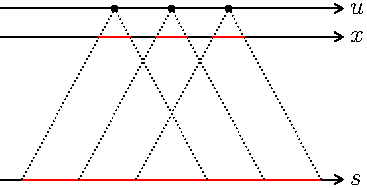
\includegraphics[scale=1]{sketches/projection_type_shifted.pdf}
  		\caption{Perspective projections, images are shifted}
   		\label{fig:perspective_shifted_projections}
	\end{subfigure}%
	\qquad
	\begin{subfigure}[b]{0.4\textwidth}
		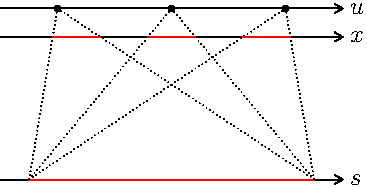
\includegraphics[scale=1]{sketches/projection_type_sheared.pdf}
		\caption{Sheared projections, cameras have a common image plane}
		\label{fig:sheared_projections}
	\end{subfigure}
	\caption{Different methods to capture a lightfield}
\end{figure}

\section{Notation}

The two-plane representation is used to describe a 4D-light field $l\left( u, v, s, t \right)$, where $\left( u, v \right)$ is the coordinate for the camera plane and $\left( s, t \right)$ for the focal plane. 

\begin{center}
	\begin{tabular}{|l|l|}
	
		\hline
		Symbol 	& Meaning \\
		\hline
		$d_c$ 	& Distance between two cameras \\ 
		
		$d_s$ 	& Distance between image plane and center of projection \\ 
		
		$z$ 	& Distance between the camera plane and the scene origin \\ 
		
		$u_j$	& Position of camera $j$ \\
		
		$x_j^i$ & Position of pixel $j$ on the image plane of camera $i$ \\
		
		$s_j^i$ & Position of pixel $j$ on layer $i$ \\ 
		
		$d_L$ 	& Distance between two layers \\ 
		\hline

	\end{tabular} 
\end{center}

\section{A first implementation for orthographic projections}	\label{sec:first_implementation}
In a first step, I (re-)implemented the tomographic light field synthesis for layered 3D-displays in MATLAB, based on the theory in \cite{WETZ_TOMO} and their publicly available MATLAB code. The core problem to solve is

\begin{equation} \label{eq:core_problem}
	\begin{aligned}
		& \underset{x}{\text{argmin}} & & \lVert Px - \bar{l} \rVert \\
		& \text{subject to} & & -\infty \leq x \leq 0,
	\end{aligned}
\end{equation}

where $\bar{l}$ is the log of the original light field $l$. The solution $x$ is in log-space as well, therefore the constraints are chosen accordingly since the layers have finite contrast, i.e. $0 \leq e^x \leq 1$.

\begin{figure}[h]
	\centering
	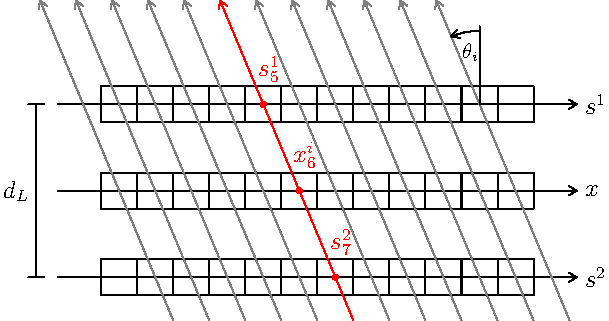
\includegraphics[scale=1]{sketches/projection_type_orthographic.pdf} 
	\caption{The rays captured by camera $i$ using orthographic projection. All rays from one camera have the same angle $\theta_i$, which is measured relative to the surface normal of the layers. $x_6^i$, $s_5^2$ and $s_7^1$ denote the intersections of the ray with the camera sensor and the layers. $d_L$ is the distance between the layers.}
	\label{fig:orthographic_cameras_layers_sketch}
\end{figure}

Figure \ref{fig:orthographic_cameras_layers_sketch} shows the way we can construct $P$. For each camera we know the angle $\theta_i$. Lets assume we have two layers. We can place the sensor plane between the two layers as shown in figure \ref{fig:orthographic_cameras_layers_sketch}. For a pixels $x^i$ on the sensor plane, we can compute the positions

\begin{align*}
	& s^1 = x^i + \frac{d_L}{2}\tan\left( \theta_i \right) && \text{and} && s^2 = s_1 - d_L \tan\left( \theta_i \right) \text{.}
\end{align*}

Once we have the positions $s^1$ and $s^2$, we compute linear indices $k$ from $\left(i, x^i\right)$, $l_1$ from $\left(s^1, 1\right)$ and $l_2$ from $\left(s^2, 2\right)$. Finally, we set $P\left(k, l_1\right) = 1$ and $P\left(k, l_2\right) = 1$. The extension for 4D-light fields and more layers is straightforward.

Having constructed the matrix $P$ which defines a system of linear equations, I used the iterative  linear least squares solver \emph{lsqlin} in MATLAB to find a solution of equation \ref{eq:core_problem}. This method turns out to be too slow when the matrix is very large. I found another iterative method called The Simultaneous Algebraic Reconstruction Technique (SART) that turns out to be efficient for my problem. It is often used in tomography applications. For the definition and convergence analysis of SART, I refer to \cite{CONV_SART}. 

\section{Moving to light fields of type 1}
The next challenge is to support light fields of type 1, as described in section \ref{sec:lftypes}. The motivation comes from the fact that most (online) light field archives provide datasets of this type. And there is also the plenoptic camera we can produce light fields with. 
\\
The requirements for this setup are the following:

\begin{itemize}
	\item A camera plane of known size/camera positions
	\item The distance from the camera plane to the scene origin: $z$
	\item The distance from the camera plane/center of projection to the sensor plane: $d_s$
	\item The field of view of the cameras
	\item The size and placement of each layer relative to the scene origin
\end{itemize}

I make the assumption that the cameras are pinhole cameras. The disparity of the images is given by $D = x_1 - x_2 = \frac{d_s d_c}{z}$, where $d_c$ is the distance between two cameras.

\subsection{Approach 1: From camera pixels to layer pixels}
My idea for this approach is to go through each pixel for each camera and trace back the ray going through this pixel and the center of projection. Knowing the ray direction, we can compute the intersection with each layer. This gives us pixel correspondences between camera pixel- and layer pixel coordinates. For the valid intersections, we would then add the value 1 in the matrix at the respective index. 
\\
This method does not seem to work. The main problem is that a lot of layer pixels may not be hit by rays for a camera. It heavily depends on the resolution of the cameras and the layers for this method to work. The problem is shown in figure \ref{fig:problem_camera_to_layers}.

\begin{figure}[t]
	\centering
	\begin{subfigure}[t]{0.4\textwidth}
 		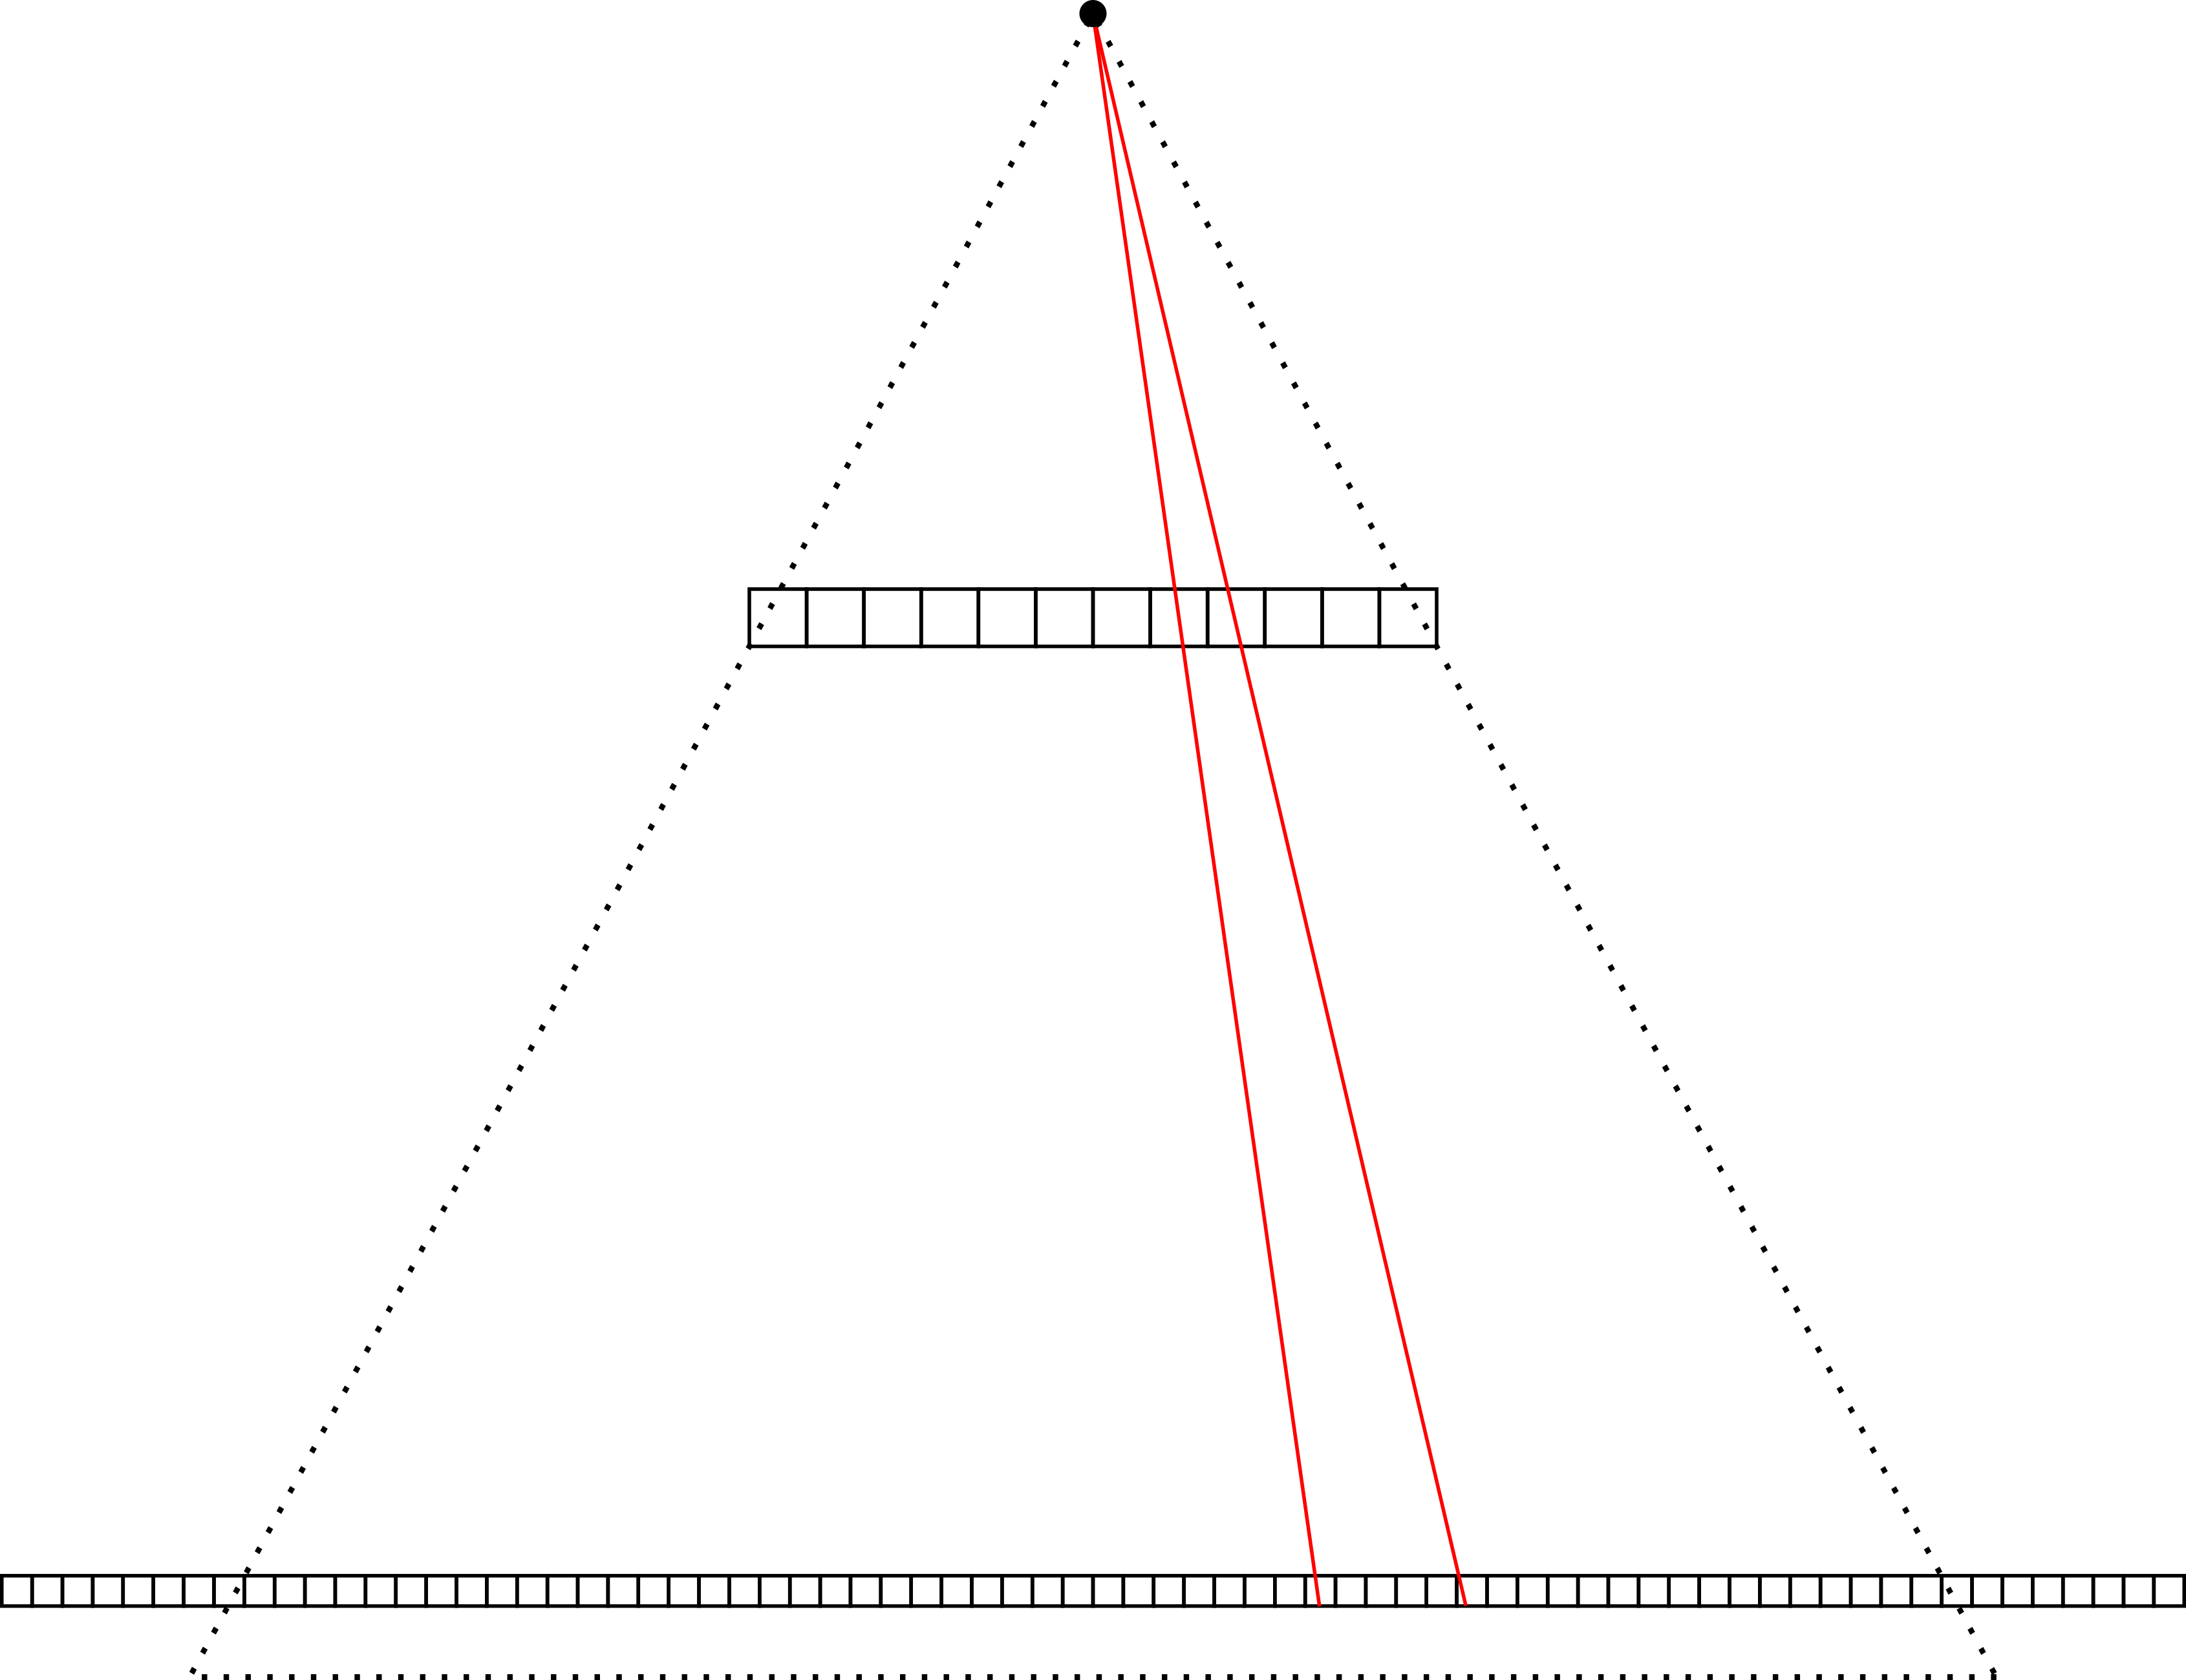
\includegraphics[scale=0.3]{sketches/problem_camera_to_layers.png} 
		\caption{Two rays hitting a cameras sensor in neighbouring pixels. The two rays intersect with the layer pixels, with multiple pixels in between.}
		\label{fig:problem_camera_to_layers}
	\end{subfigure}%
	\qquad
	\begin{subfigure}[t]{0.4\textwidth}
		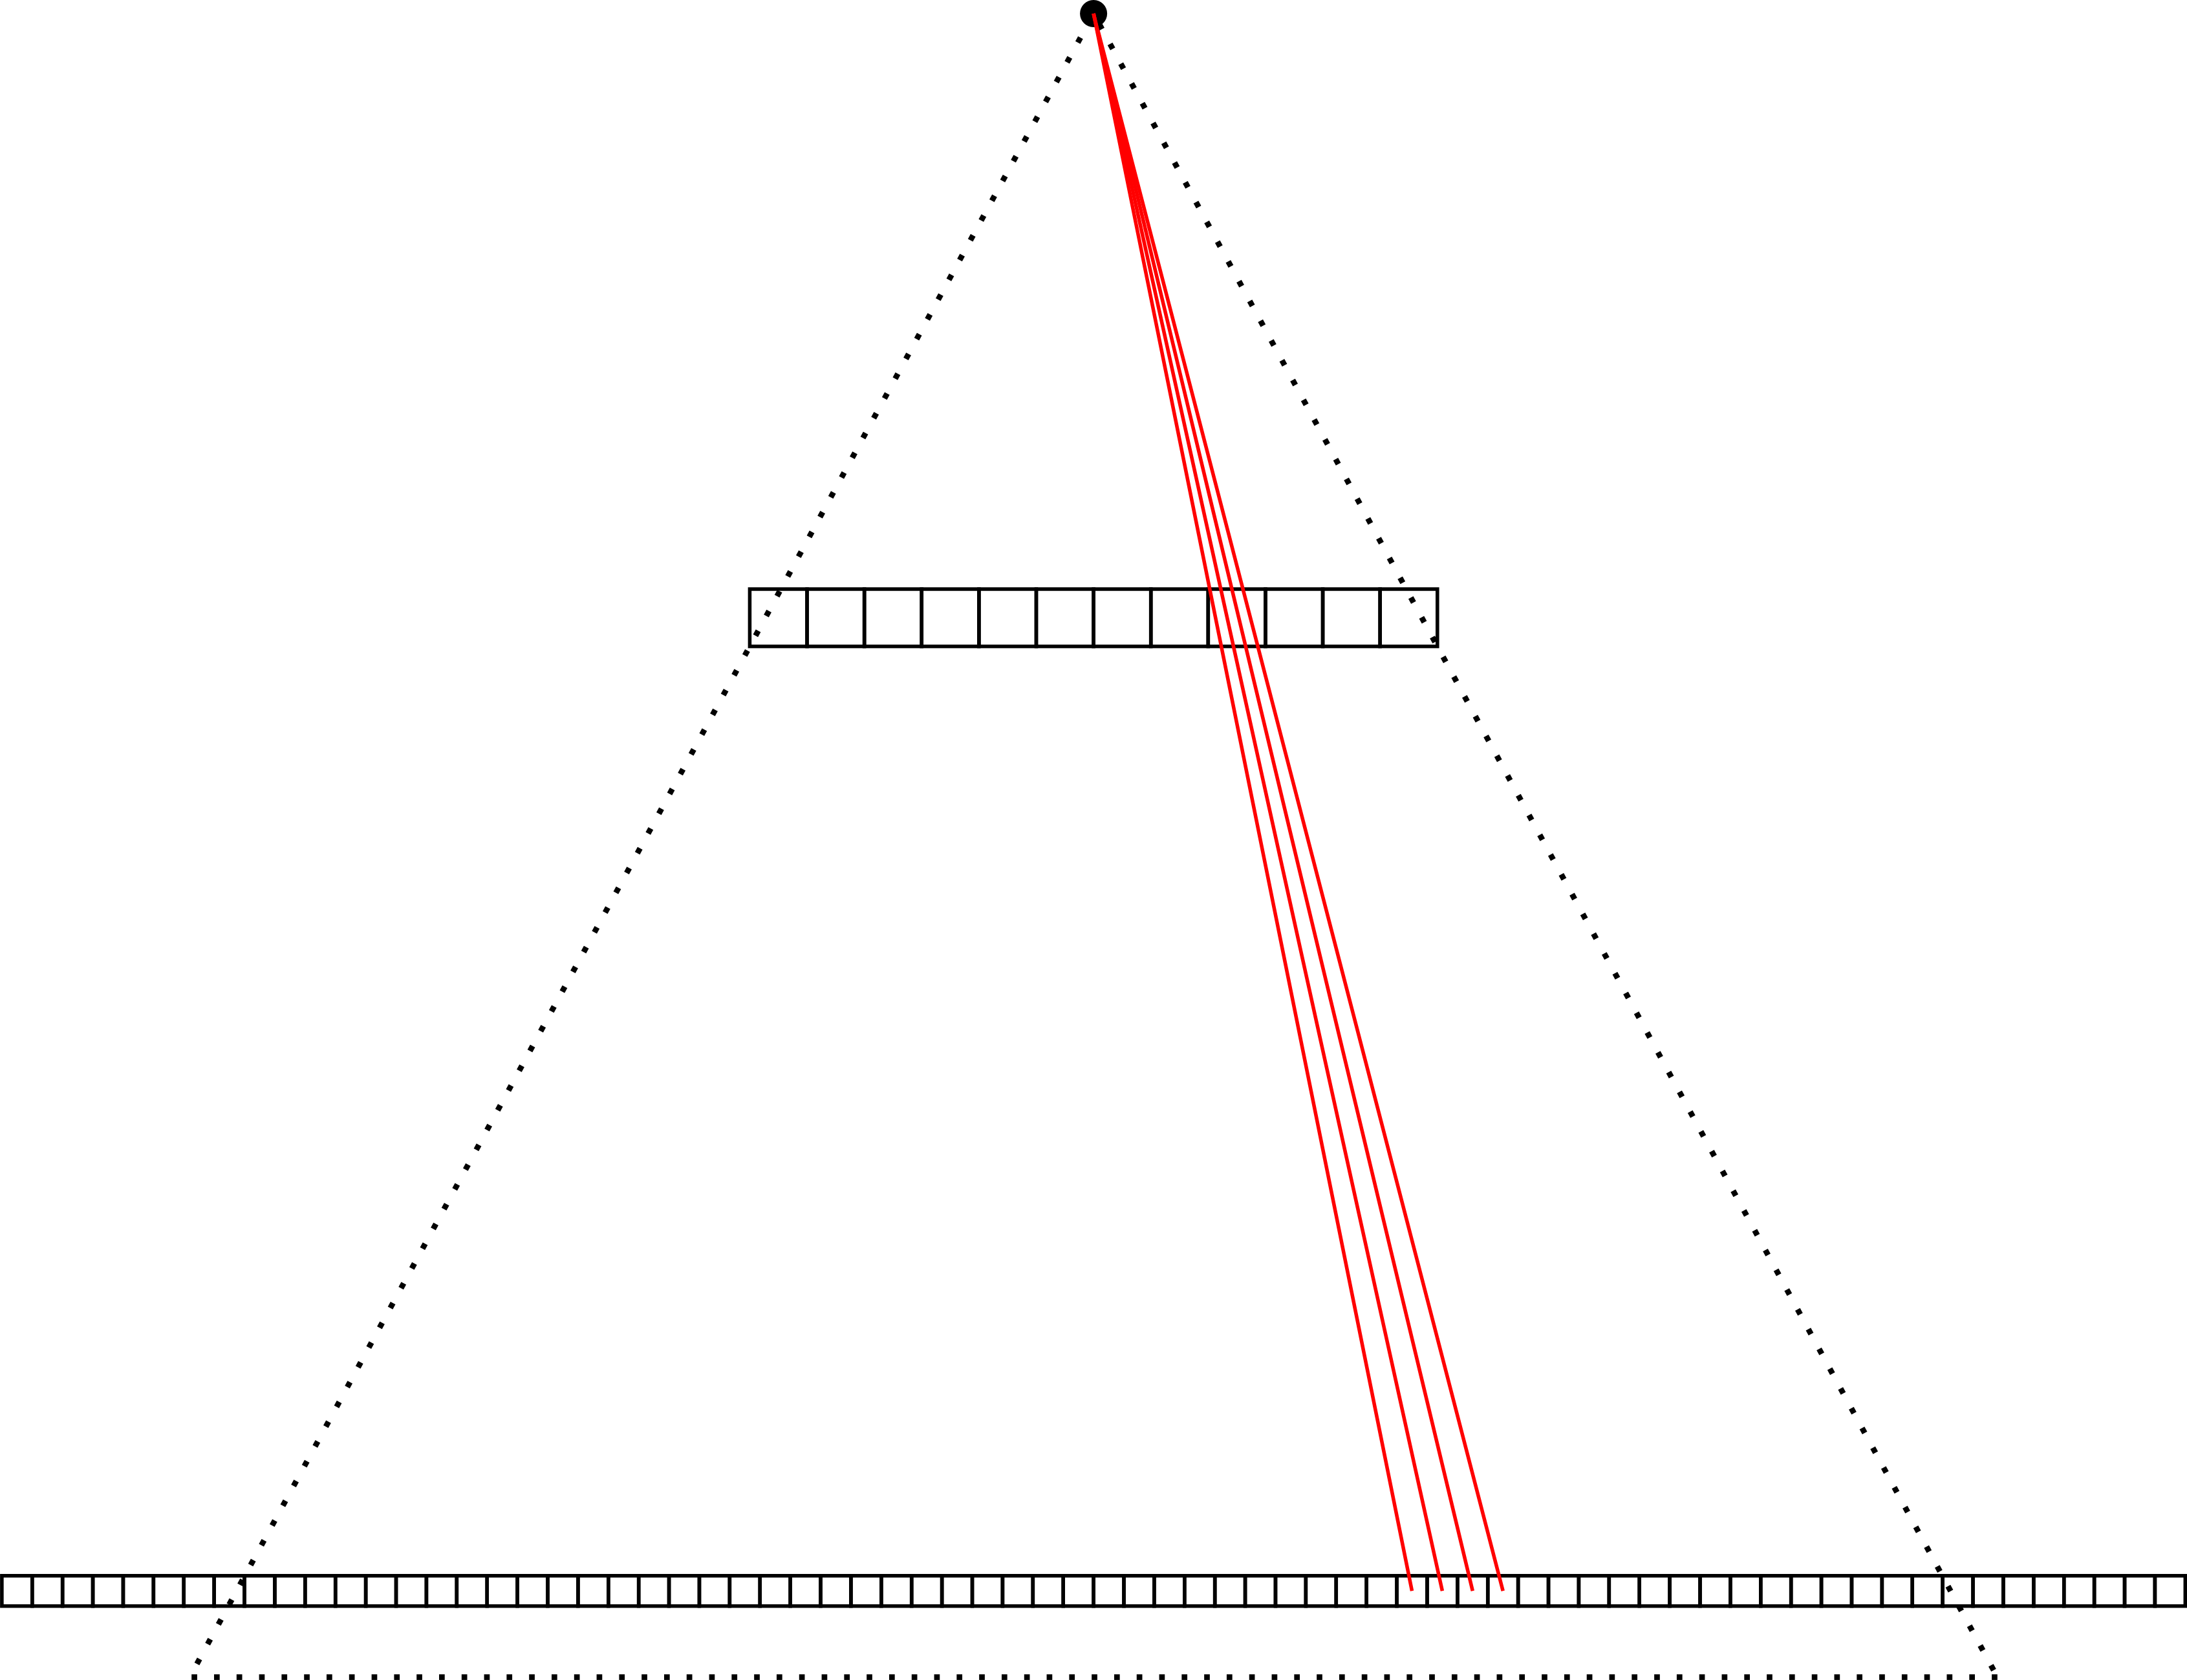
\includegraphics[scale=0.3]{sketches/problem_layers_to_camera_rounding.png}
		\caption{Rays coming from four different layer pixels and hitting the same sensor pixel in the camera.}
		\label{fig:problem_layers_to_camera}
	\end{subfigure}
	\caption{Problems that can arise from different resolution in image- and layer space.}
\end{figure}

\subsection{Approach 2: Converting the light field}
The next idea is to reparametrize the light field $l \left( c_y, c_x, y, x \right)$ to an angular representation $l' \left( \theta_y, \theta_x, v, u \right)$. Here, the number of angles corresponds to the resolution of the camera sensor. The motivation behind this approach is that we can fix 
$\left( \theta_y, \theta_x \right)$ in the latter representation and get an orthogonal view. We would then plug this light field into the old algorithm to solve for the layers.
\\
For the reparametrization, we construct matrices

\begin{align*}
	C_y \left( \theta_y, :, v, : \right) && C_x \left( :, \theta_x, :, u \right) && I_y \left(\theta_y, :, v, : \right) && I_x \left( :, \theta_x, : u \right) 
\end{align*}

of the same dimension as the light field resolution. The ":" represents replication of the matrix in the respective dimension. We use these matrices to obtain a interpolated light field $l' \left( \theta_y, \theta_x, v, u \right)$.
\\\\ TODO: Why didn't it work in the end? 

\subsection{Approach 3: From layer pixels to camera pixels}
This idea is basically the opposite of approach 1. For every layer pixel and for every camera we compute the ray intersection on the sensor plane. The positions $x_j^1$ and $x_j^2$ shown in figure \ref{fig:cameras_layers_sketch} are computed as follows:

\begin{align*}
	& x_j^1 = \left( s_i^1 - u_1 \right) \frac{d_s}{z + d_L} & x_k^2 = \left( s_i^1 - u_2 \right) \frac{d_s}{z + d_L}
\end{align*}

These points will be scaled and rounded to their corresponding pixels. We can then construct the propagation matrix $P$ the same way as in section \ref{sec:first_implementation}.
As demonstrated in figure \ref{fig:problem_layers_to_camera}, it often happens that a patch of layer pixels gets mapped to the same camera pixel due to rounding and thus, one pixel from the camera would contribute to multiple layer pixels. This also results in high column sums of the matrix $P$ from equation \ref{eq:core_problem}.

\begin{figure}[h]
	\centering
	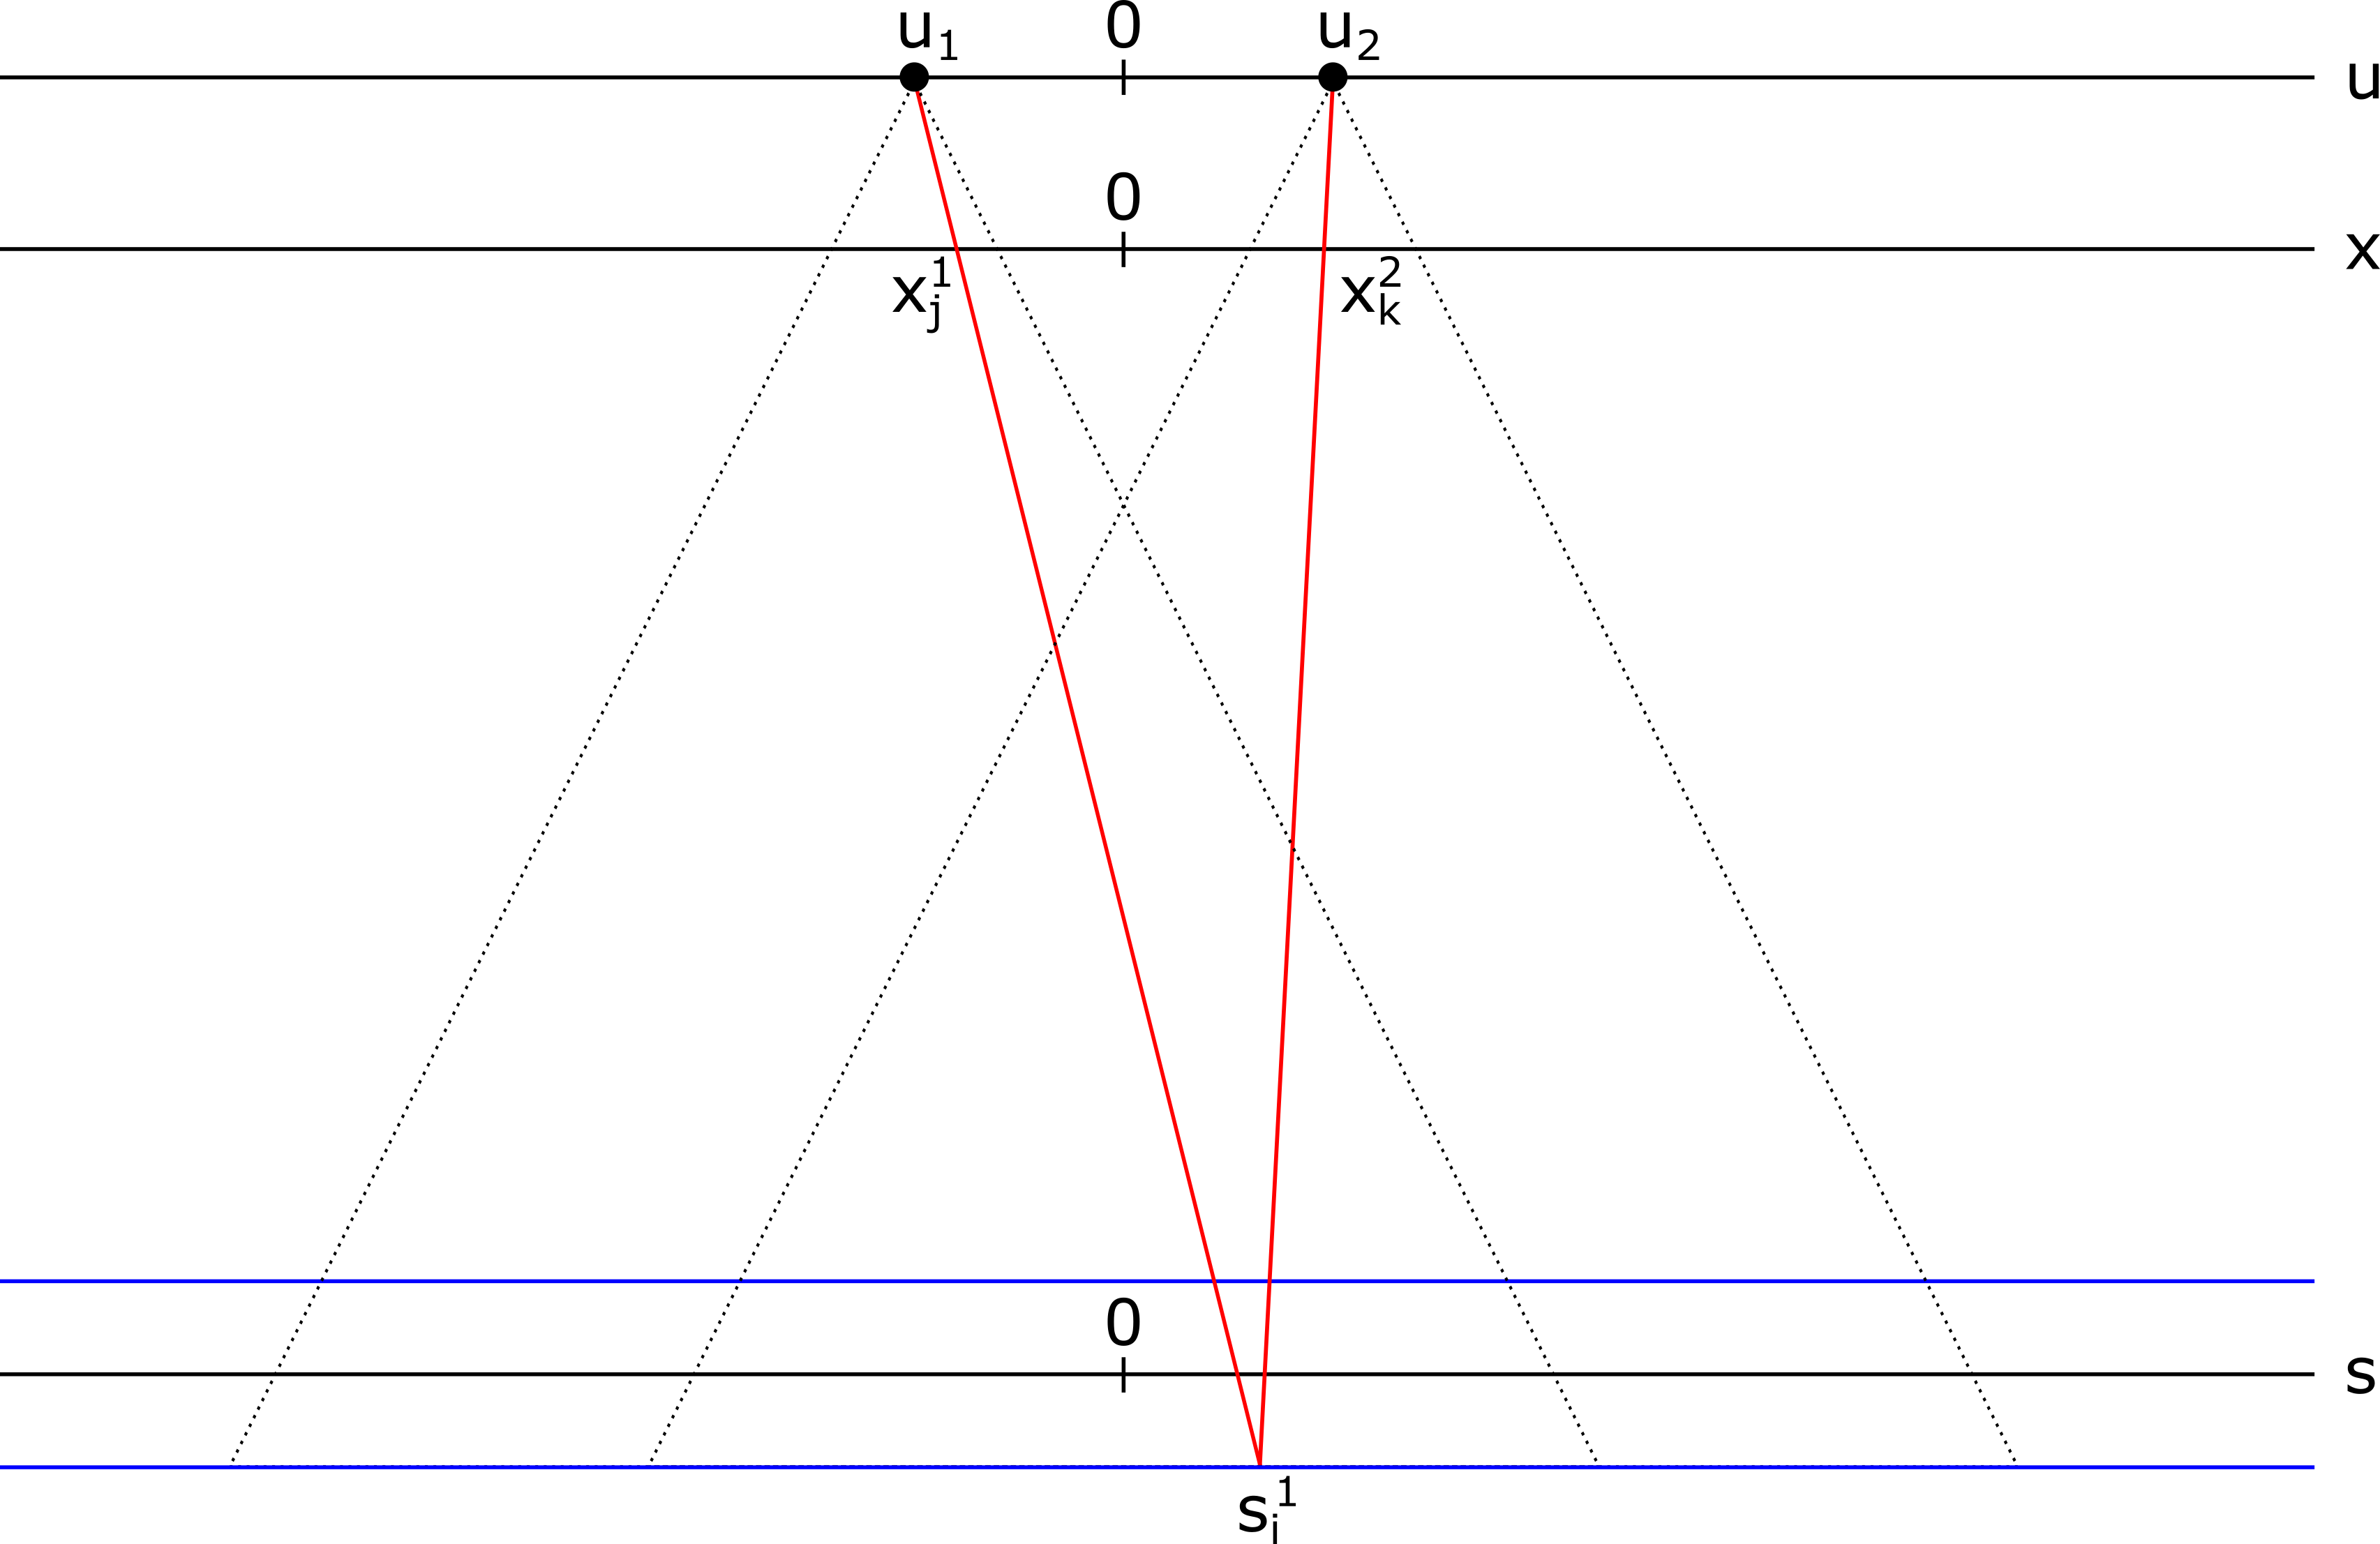
\includegraphics[scale=0.5]{sketches/camera_layers_sketch.png} 
	\caption{Two rays (red) intersecting the first layer (blue) at position $s_i^1$. The rays are captured by different cameras at positions $u_1$ and $u_2$, hitting the camera sensor at locations $x_j^1$ and $x_k^2$. The dotted lines represent the field of view of each camera.}
	\label{fig:cameras_layers_sketch}
\end{figure}

\section{Creating synthetic light fields}
I used light fields from the Heidelberg and Stanford light field archives. In addition, I also rendered synthetic scenes with POV-Ray. The advantage of a synthetic light field is that the cameras can be precisely placed and all the required parameters are known and can be adjusted easily. 

\newpage
\section{Review of the two implementations}
\subsection{Orthographic projections}

\begin{figure}[h]
	\centering
	\begin{subfigure}[c]{\textwidth}
 		\includegraphics[width=\textwidth]{results/dice_orthographic_rec_fov10_blurry_3Layers/P_full.eps}
  		\caption{Full matrix.}
   		\label{fig:P_orthographic_full}
	\end{subfigure}%
	\\
	\begin{subfigure}[c]{\textwidth}
		\includegraphics[width=\textwidth]{results/dice_orthographic_rec_fov10_blurry_3Layers/P1-10000_1-1000.eps}
		\caption{The upper left section of the matrix.}
		\label{fig:P_orthographic_section}
	\end{subfigure}
	\caption{The structure of the propagation matrix $P$. The non-zero elements are marked as blue.}
\end{figure}

\newpage

\begin{figure}[h]
	\centering
	\begin{subfigure}[c]{0.3\textwidth}
 		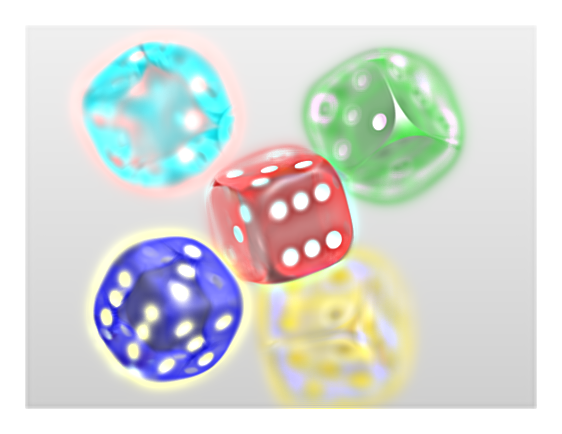
\includegraphics[width=\textwidth]{results/dice_orthographic_rec_fov10_blurry_3Layers/1.png}
  		\caption{Layer 1}
	\end{subfigure}%
	~
	\begin{subfigure}[c]{0.3\textwidth}
		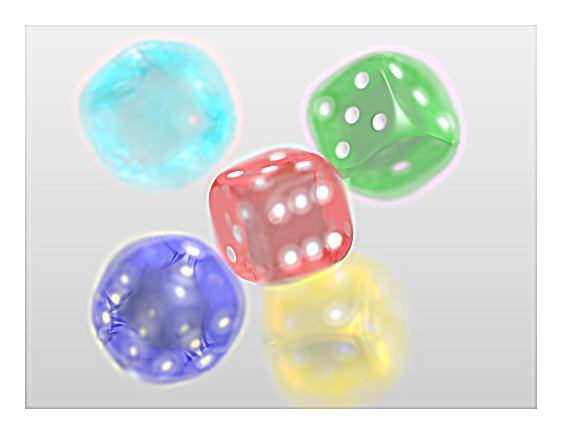
\includegraphics[width=\textwidth]{results/dice_orthographic_rec_fov10_blurry_3Layers/2.png}
		\caption{Layer 2}
	\end{subfigure}%
	~
	\begin{subfigure}[c]{0.3\textwidth}
		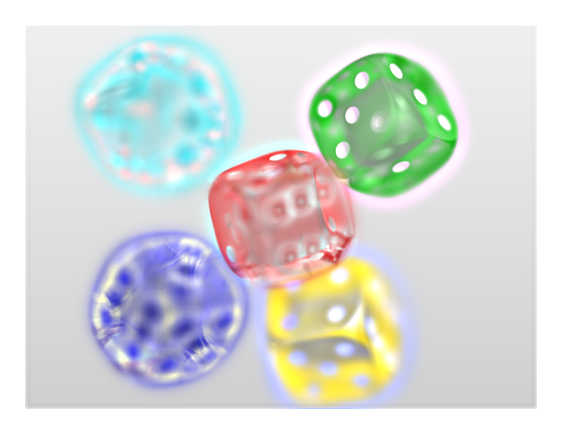
\includegraphics[width=\textwidth]{results/dice_orthographic_rec_fov10_blurry_3Layers/3.png}
		\caption{Layer 3}
	\end{subfigure}%
	\\
	\begin{subfigure}[t]{0.4\textwidth}
		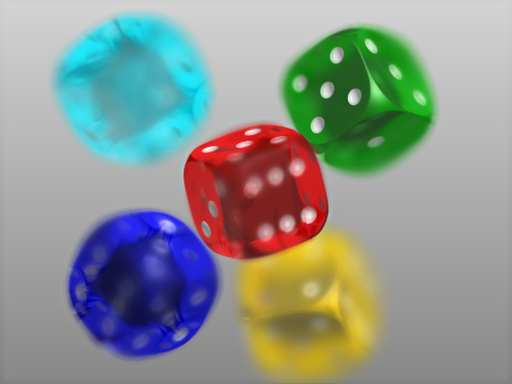
\includegraphics[width=\textwidth]{results/dice_orthographic_rec_fov10_blurry_3Layers/central_view_reconstruction.png}
		\caption{The reconstructed central view $\left( 4, 4 \right)$.}
	\end{subfigure}%
	~
	\begin{subfigure}[t]{0.4\textwidth}
		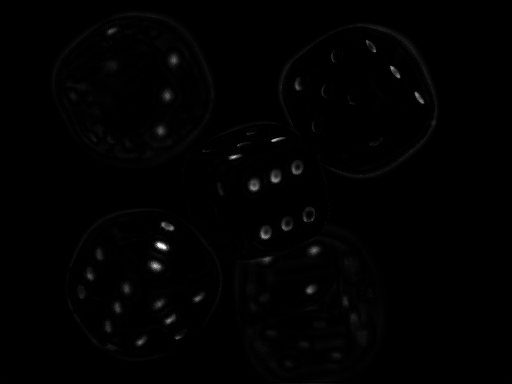
\includegraphics[width=\textwidth]{results/dice_orthographic_rec_fov10_blurry_3Layers/central_view_error.png}
		\caption{The error of the central view.}
	\end{subfigure}%
	\\
	\begin{subfigure}[t]{0.4\textwidth}
		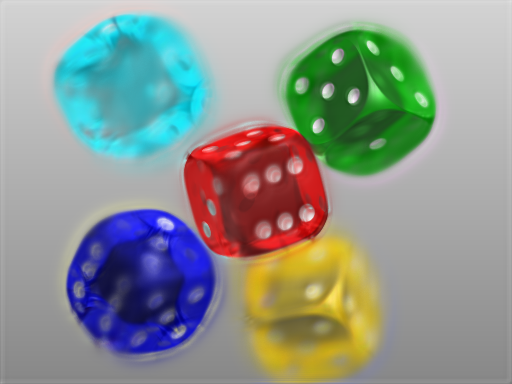
\includegraphics[width=\textwidth]{results/dice_orthographic_rec_fov10_blurry_3Layers/custom_view_reconstruction.png}
		\caption{Reconstruction of the view $\left( 7, 7 \right)$, the bottom-rightmost view.}
	\end{subfigure}%
	~
	\begin{subfigure}[t]{0.4\textwidth}
		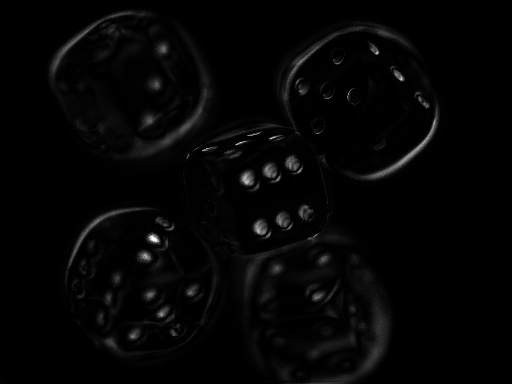
\includegraphics[width=\textwidth]{results/dice_orthographic_rec_fov10_blurry_3Layers/custom_view_error.png}
		\caption{The error of the view $\left( 7, 7 \right)$.}
	\end{subfigure}

	\caption{Optimization for three layers. The light field has an angular resolution of $7\times 7$ views. The blur in the reconstruction is also in the original light field.}
\end{figure}

\clearpage
\subsection{Perspective projections}

\begin{figure}[h]
	\centering
	\begin{subfigure}[c]{0.3\textwidth}
 		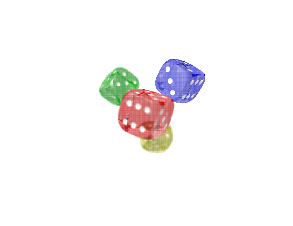
\includegraphics[width=\textwidth]{results/dice_perspective_rec_3Layers_r=0/1.png}
  		\caption{Layer 1}
	\end{subfigure}%
	~
	\begin{subfigure}[c]{0.3\textwidth}
		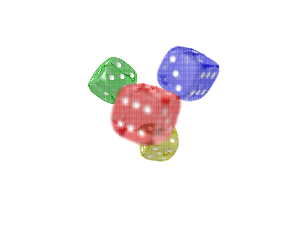
\includegraphics[width=\textwidth]{results/dice_perspective_rec_3Layers_r=0/2.png}
		\caption{Layer 2}
	\end{subfigure}%
	~
	\begin{subfigure}[c]{0.3\textwidth}
		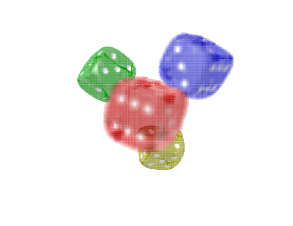
\includegraphics[width=\textwidth]{results/dice_perspective_rec_3Layers_r=0/3.png}
		\caption{Layer 3}
	\end{subfigure}%
	\\
	\begin{subfigure}[t]{0.4\textwidth}
		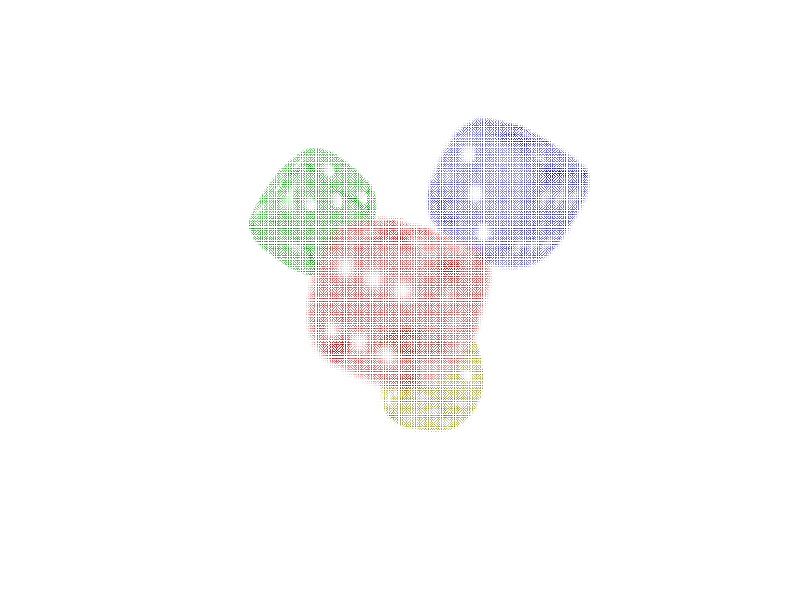
\includegraphics[width=\textwidth]{results/dice_perspective_rec_3Layers_r=0/central_view_reconstruction3-3.png}
		\caption{The reconstructed central view $\left( 3, 3 \right)$.}
	\end{subfigure}%
	~
	\begin{subfigure}[t]{0.4\textwidth}
		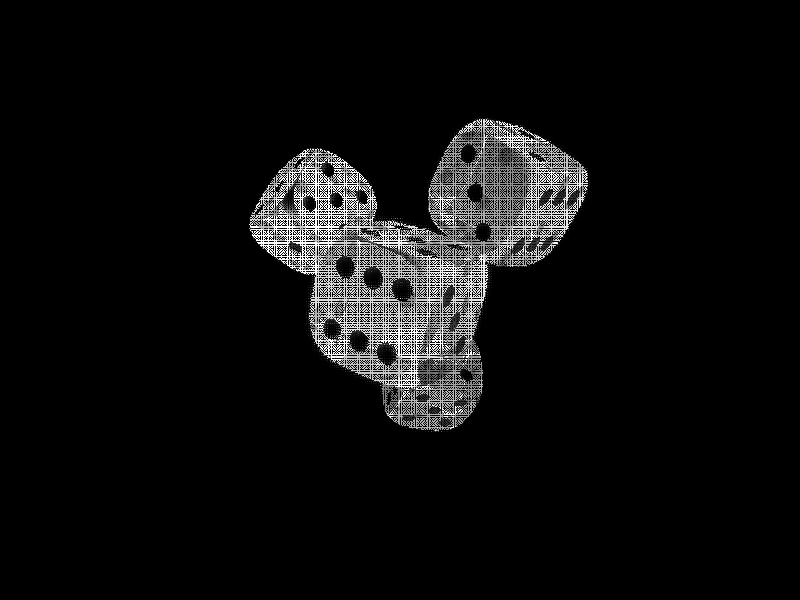
\includegraphics[width=\textwidth]{results/dice_perspective_rec_3Layers_r=0/central_view_error.png}
		\caption{The error of the central view.}
	\end{subfigure}%
	\\
	\begin{subfigure}[t]{0.4\textwidth}
		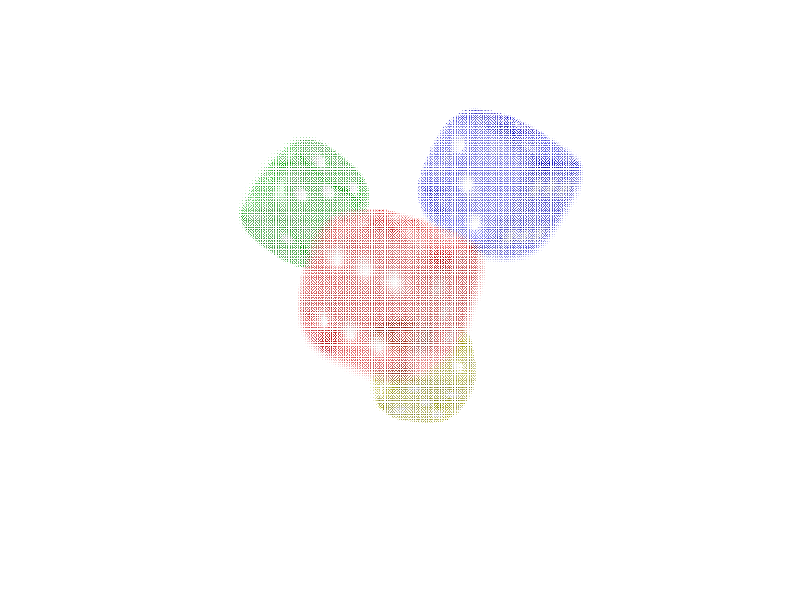
\includegraphics[width=\textwidth]{results/dice_perspective_rec_3Layers_r=0/custom_view_reconstruction5-5.png}
		\caption{Reconstruction of the view $\left( 5, 5 \right)$, the bottom-rightmost view.}
	\end{subfigure}%
	~
	\begin{subfigure}[t]{0.4\textwidth}
		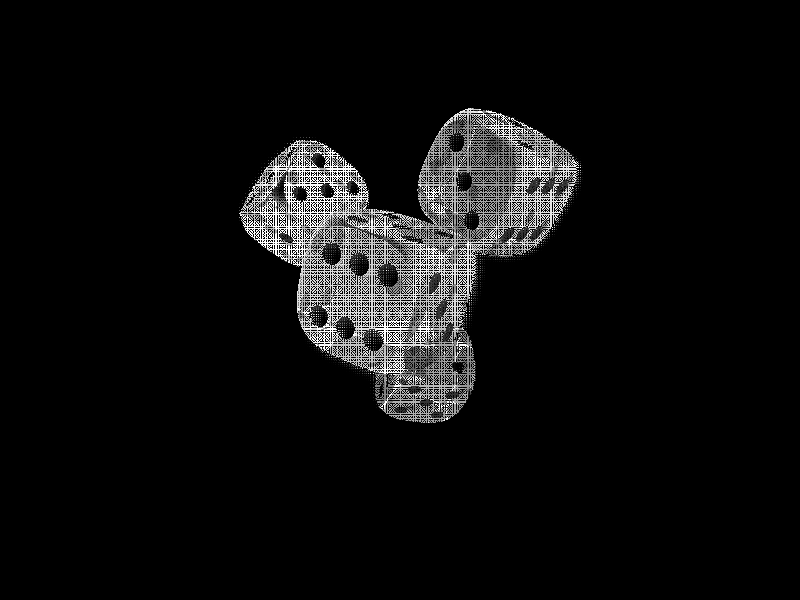
\includegraphics[width=\textwidth]{results/dice_perspective_rec_3Layers_r=0/custom_view_error.png}
		\caption{The error of the view $\left( 5, 5 \right)$.}
	\end{subfigure}%
	\\
	\begin{subfigure}[t]{0.4\textwidth}
		\begin{tabular}{|l|l|l|}
			\hline 
			View & orthographic & perspective \\ 
			\hline 
			$\left(3, 3\right)$ & ? & 54.925458 \\ 
			\hline 
			$\left(5, 5\right)$ & ? & 127.421736 \\ 
			\hline 
		\end{tabular} 
		\caption{Root-mean-square-error between the original and the reconstructed view.}
	\end{subfigure}
	\caption{Optimization for three layers. The light field has an angular resolution of $5\times 5$ views. Parameters: $z = 8$, $d_c = \left( 0.05, 0.05 \right)$, $\text{fov} = \left( 60^\circ, 45^\circ \right)$, $d_L = 1.5$}
\end{figure}


\clearpage
\begin{figure}[h]
	\centering
	\begin{subfigure}[c]{0.3\textwidth}
 		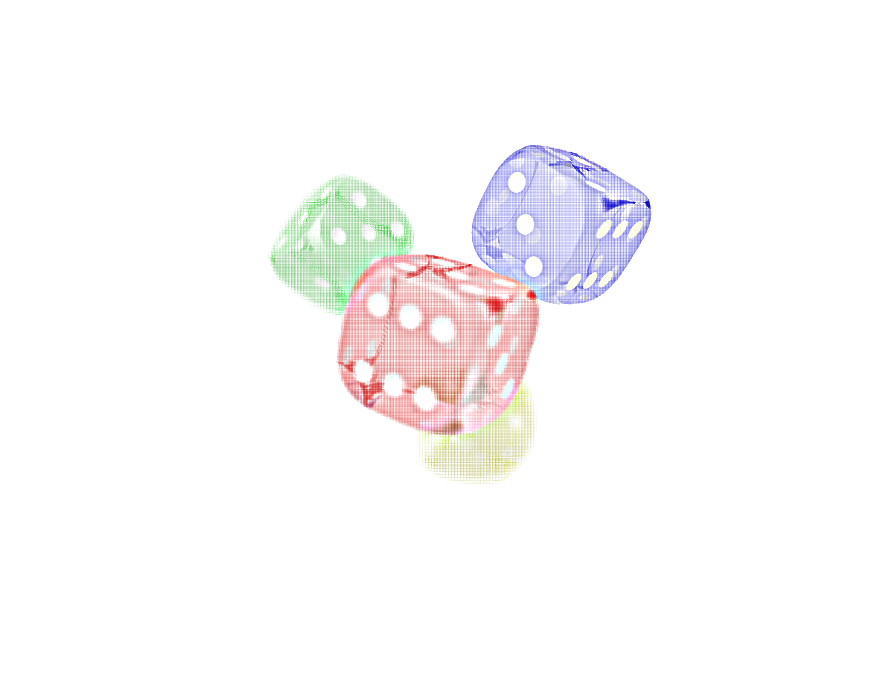
\includegraphics[width=\textwidth]{results/dice_perspective_rec_3Layers_r=1/1.png}
  		\caption{Layer 1}
	\end{subfigure}%
	~
	\begin{subfigure}[c]{0.3\textwidth}
		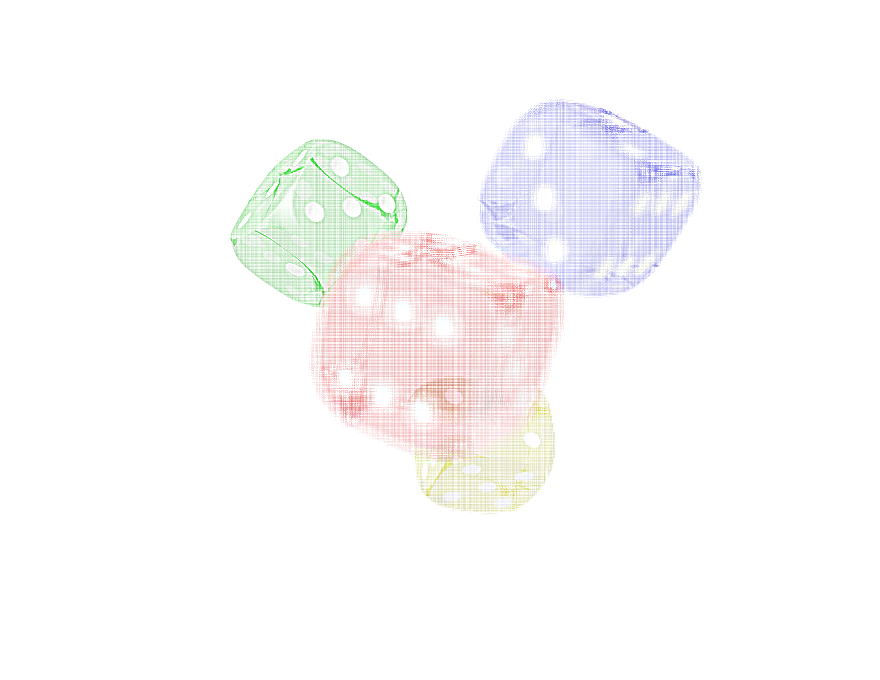
\includegraphics[width=\textwidth]{results/dice_perspective_rec_3Layers_r=1/2.png}
		\caption{Layer 2}
	\end{subfigure}%
	~
	\begin{subfigure}[c]{0.3\textwidth}
		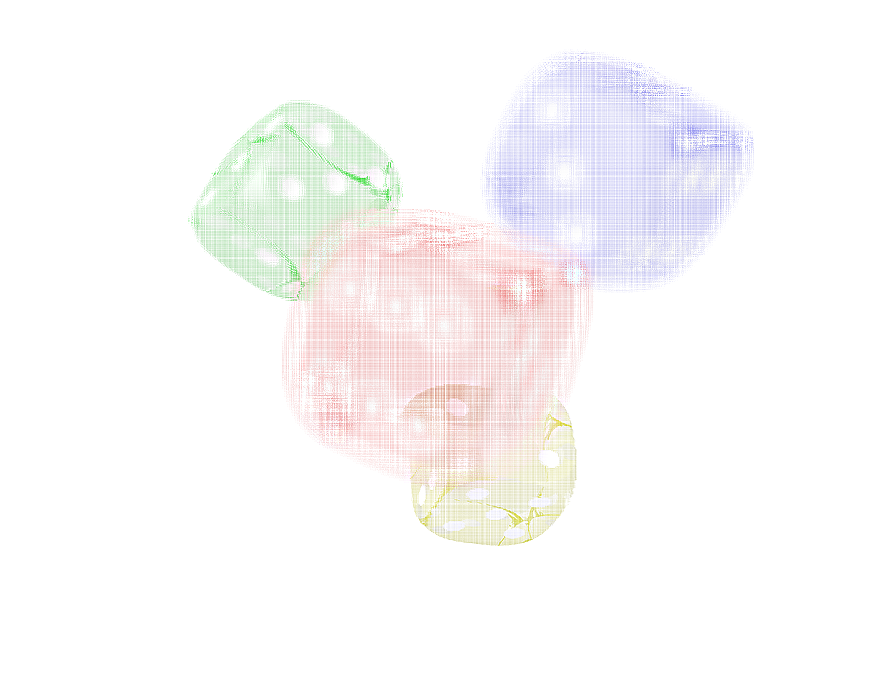
\includegraphics[width=\textwidth]{results/dice_perspective_rec_3Layers_r=1/3.png}
		\caption{Layer 3}
	\end{subfigure}%
	\\
	\begin{subfigure}[t]{0.4\textwidth}
		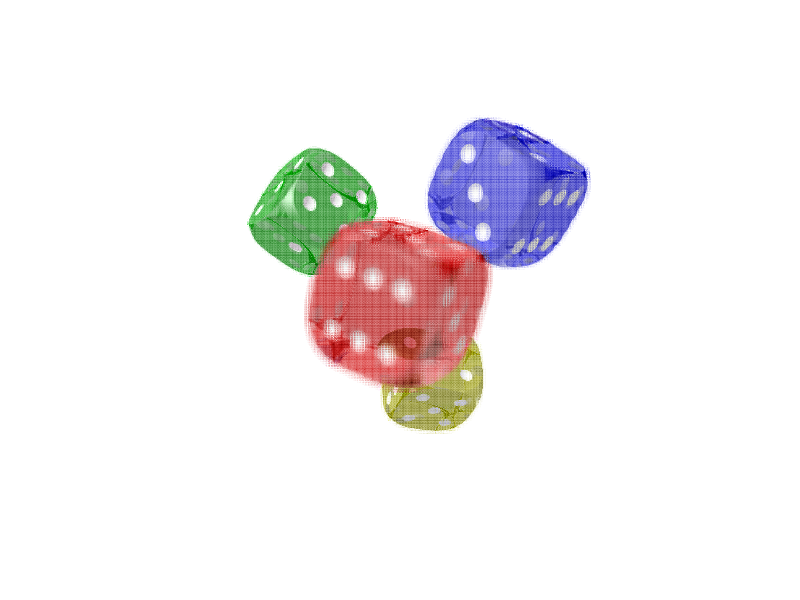
\includegraphics[width=\textwidth]{results/dice_perspective_rec_3Layers_r=1/central_view_reconstruction.png}
		\caption{The reconstructed central view $\left( 3, 3 \right)$.}
	\end{subfigure}%
	~
	\begin{subfigure}[t]{0.4\textwidth}
		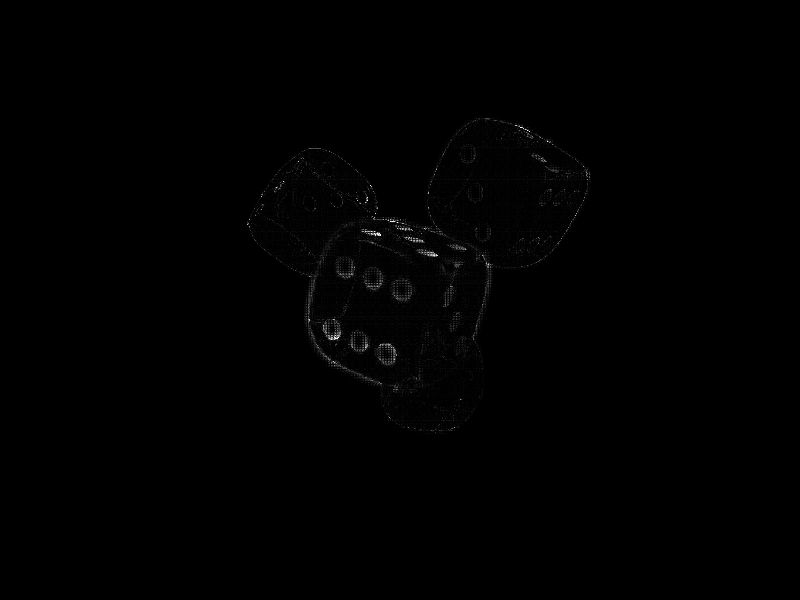
\includegraphics[width=\textwidth]{results/dice_perspective_rec_3Layers_r=1/central_view_error.png}
		\caption{The error of the central view.}
	\end{subfigure}%
	\\
	\begin{subfigure}[t]{0.4\textwidth}
		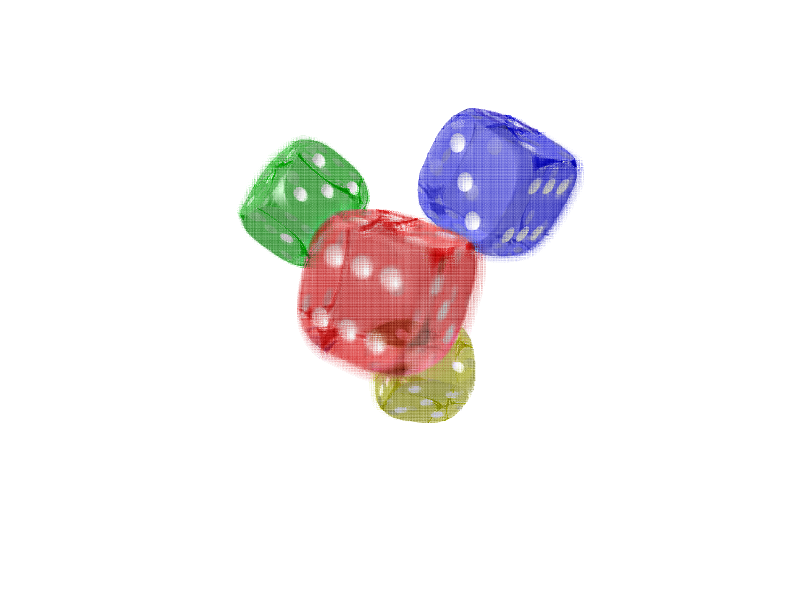
\includegraphics[width=\textwidth]{results/dice_perspective_rec_3Layers_r=1/custom_view_reconstruction.png}
		\caption{Reconstruction of the view $\left( 5, 5 \right)$, the bottom-rightmost view.}
	\end{subfigure}%
	~
	\begin{subfigure}[t]{0.4\textwidth}
		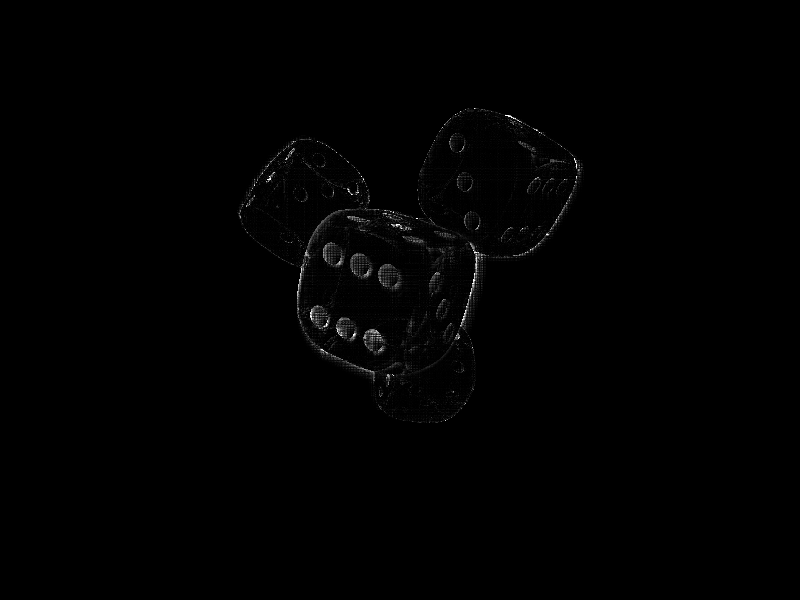
\includegraphics[width=\textwidth]{results/dice_perspective_rec_3Layers_r=1/custom_view_error.png}
		\caption{The error of the view $\left( 5, 5 \right)$.}
	\end{subfigure}

	\caption{Optimization for three layers. The light field has an angular resolution of $5\times 5$ views.}
\end{figure}

\newpage
\begin{figure}[h]
	\centering
	\begin{subfigure}[c]{0.3\textwidth}
 		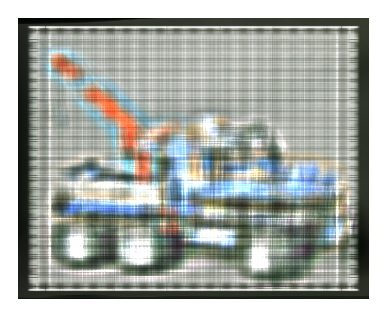
\includegraphics[width=\textwidth]{results/legotruck_perspective_rec_3Layers_r=0/1.png}
  		\caption{Layer 1}
	\end{subfigure}%
	~
	\begin{subfigure}[c]{0.3\textwidth}
		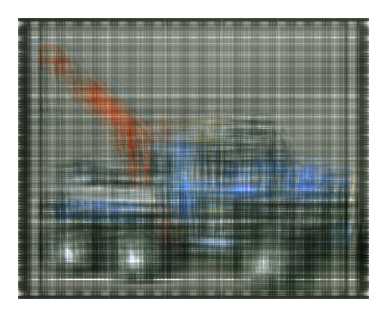
\includegraphics[width=\textwidth]{results/legotruck_perspective_rec_3Layers_r=0/2.png}
		\caption{Layer 2}
	\end{subfigure}%
	~
	\begin{subfigure}[c]{0.3\textwidth}
		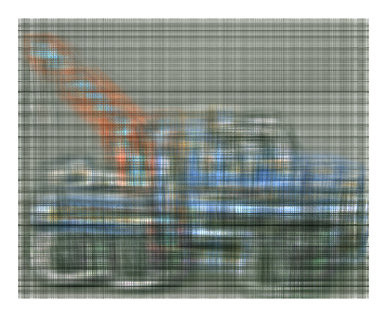
\includegraphics[width=\textwidth]{results/legotruck_perspective_rec_3Layers_r=0/3.png}
		\caption{Layer 3}
	\end{subfigure}%
	\\
	\begin{subfigure}[t]{0.4\textwidth}
		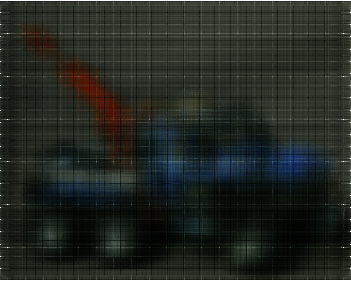
\includegraphics[width=\textwidth]{results/legotruck_perspective_rec_3Layers_r=0/central_view_reconstruction5-5.png}
		\caption{The reconstructed central view $\left( 5, 5 \right)$.}
	\end{subfigure}%
	~
	\begin{subfigure}[t]{0.4\textwidth}
		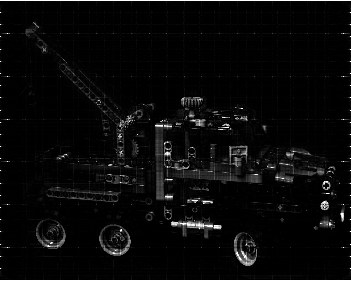
\includegraphics[width=\textwidth]{results/legotruck_perspective_rec_3Layers_r=0/central_view_error.png}
		\caption{The error of the central view.}
	\end{subfigure}%
	\\
	\begin{subfigure}[t]{0.4\textwidth}
		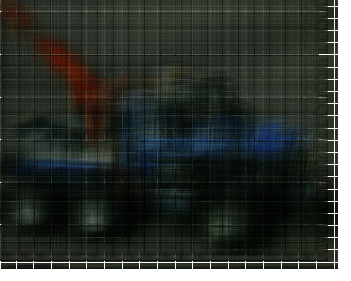
\includegraphics[width=\textwidth]{results/legotruck_perspective_rec_3Layers_r=0/custom_view_reconstruction9-9.png}
		\caption{Reconstruction of the view $\left( 9, 9 \right)$, the bottom-rightmost view.}
	\end{subfigure}%
	~
	\begin{subfigure}[t]{0.4\textwidth}
		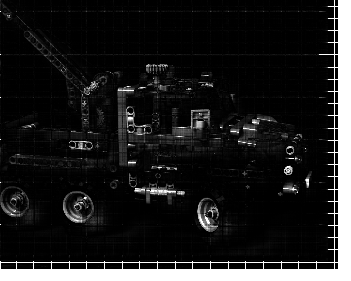
\includegraphics[width=\textwidth]{results/legotruck_perspective_rec_3Layers_r=0/custom_view_error.png}
		\caption{The error of the view $\left( 9, 9 \right)$.}
	\end{subfigure}

	\caption{Optimization for three layers. The light field has an angular resolution of $9\times 9$ views.}
	\label{fig:legotruck_artefacts_r=0}
\end{figure}


\newpage
\begin{figure}[h]
	\centering
	\begin{subfigure}[c]{0.3\textwidth}
 		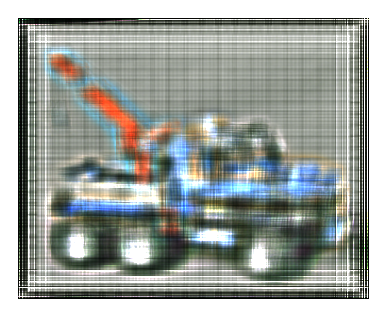
\includegraphics[width=\textwidth]{results/legotruck_perspective_rec_3Layers_r=1/1.png}
  		\caption{Layer 1}
	\end{subfigure}%
	~
	\begin{subfigure}[c]{0.3\textwidth}
		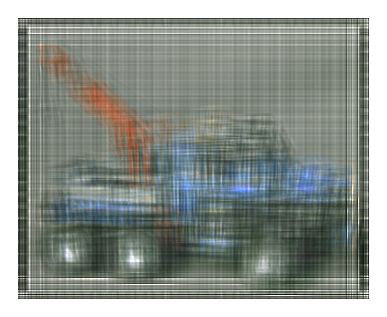
\includegraphics[width=\textwidth]{results/legotruck_perspective_rec_3Layers_r=1/2.png}
		\caption{Layer 2}
	\end{subfigure}%
	~
	\begin{subfigure}[c]{0.3\textwidth}
		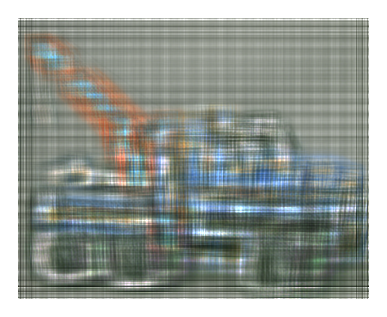
\includegraphics[width=\textwidth]{results/legotruck_perspective_rec_3Layers_r=1/3.png}
		\caption{Layer 3}
	\end{subfigure}%
	\\
	\begin{subfigure}[t]{0.4\textwidth}
		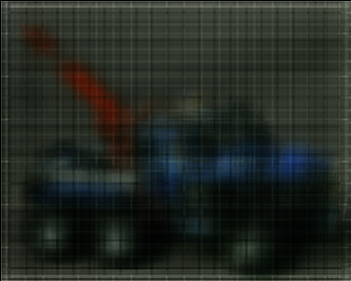
\includegraphics[width=\textwidth]{results/legotruck_perspective_rec_3Layers_r=1/central_view_reconstruction5-5.png}
		\caption{The reconstructed central view $\left( 5, 5 \right)$.}
	\end{subfigure}%
	~
	\begin{subfigure}[t]{0.4\textwidth}
		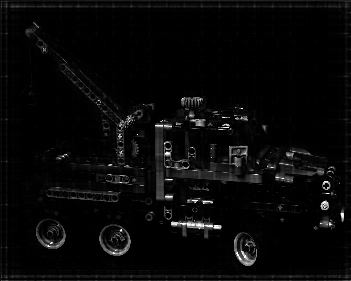
\includegraphics[width=\textwidth]{results/legotruck_perspective_rec_3Layers_r=1/central_view_error.png}
		\caption{The error of the central view.}
	\end{subfigure}%
	\\
	\begin{subfigure}[t]{0.4\textwidth}
		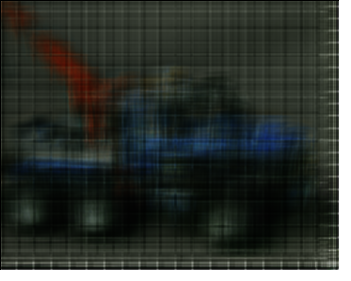
\includegraphics[width=\textwidth]{results/legotruck_perspective_rec_3Layers_r=1/custom_view_reconstruction9-9.png}
		\caption{Reconstruction of the view $\left( 9, 9 \right)$, the bottom-rightmost view.}
	\end{subfigure}%
	~
	\begin{subfigure}[t]{0.4\textwidth}
		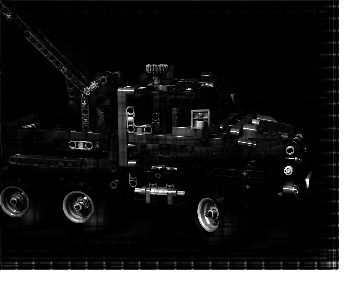
\includegraphics[width=\textwidth]{results/legotruck_perspective_rec_3Layers_r=1/custom_view_error.png}
		\caption{The error of the view $\left( 9, 9 \right)$.}
	\end{subfigure}

	\caption{Optimization for three layers. The light field has an angular resolution of $9\times 9$ views.}
\end{figure}

\clearpage
\section{Fixing the artefacts that occur in the reconstruction}

\begin{figure}[h]
	\centering
	\begin{subfigure}[t]{0.4\textwidth}
 		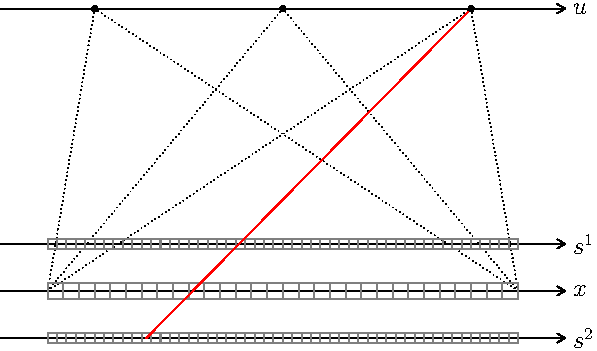
\includegraphics[width=\textwidth]{sketches/sheared_projections_layers_overview-1.pdf} 
  		\caption{Ray (red) coming from a pixel on layer $s^2$ intersecting the sensor plane $x$ and the topmost  layer $s^1$. }
  		\label{fig:intersections_and_weights_overview}
	\end{subfigure}%
	\quad
	\begin{subfigure}[t]{0.4\textwidth}
		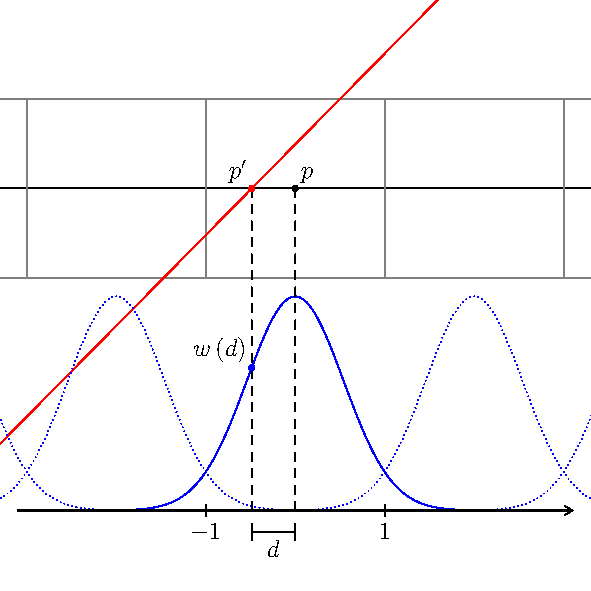
\includegraphics[width=\textwidth]{sketches/sheared_projections_layers_overview-2.pdf} 
  		\caption{The ray intersects at $p'$. The nearest pixel with center $p$ is considered and a weight $w\left(d\right)$ is computed from the deviation $d = p - p'$.}
	\end{subfigure}%
	\caption{Calculation of the intersections and weights.}
	\label{fig:intersections_and_weights}
\end{figure}

The main idea is to use a kernel to weight the ray-pixel-correspondences. As depicted in figure \ref{fig:intersections_and_weights}, the weight is computed from the deviation of the pixel center. For any ray, the nearest pixel gets selected and a weight is calculated. I considered and tested the following configurations:

\begin{itemize}
	\item 	Weights only for the sensor plane $x$
	\item 	Combination of weights on sensor plane and each layer
	\item 	Box-Filter for the sensor plane only
	\item	Combination of Box-Filter on sensor plane and each layer
\end{itemize}

During the implementation of the box-filter it came to my attention that the propagation matrix $P$ should be normalized along the rows. This normalization alone seems to have a drastic impact on the artefacts we encountered. Figure \ref{fig:normalization_impact_comparison} compares the impact of normalization on the reconstruction quality. Notice that figure \ref{fig:normalization_no_weights} shows the best result, albeit no weights were calculated, and all other settings have no visible influence. The conclusion is: Adding weights to the system seems to have little to no impact on the optimization of the layers and the reconstruction quality. 
\newline
It is also worth noticing that the row-normalization cancels out the sensor weights. This is due to the fact that during the construction of $P$, each entry (layer weight) of a row gets multiplied by the corresponding sensor weight.

\begin{figure}[h]
	\centering
	\begin{subfigure}[t]{0.45\textwidth}
 		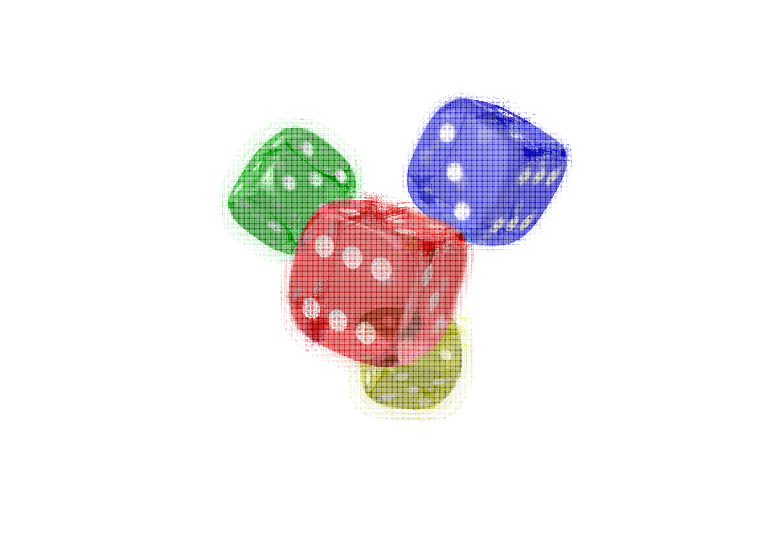
\includegraphics[width=\textwidth]{results/aliasing_fixes/compare_normalization/no_normalization_r=0_weights=1/central_view_reconstruction2-2.png} 
  		\caption{No normalization, box radius $0$, $w \equiv 1$.}
	\end{subfigure}%
	~
	\begin{subfigure}[t]{0.45\textwidth}
		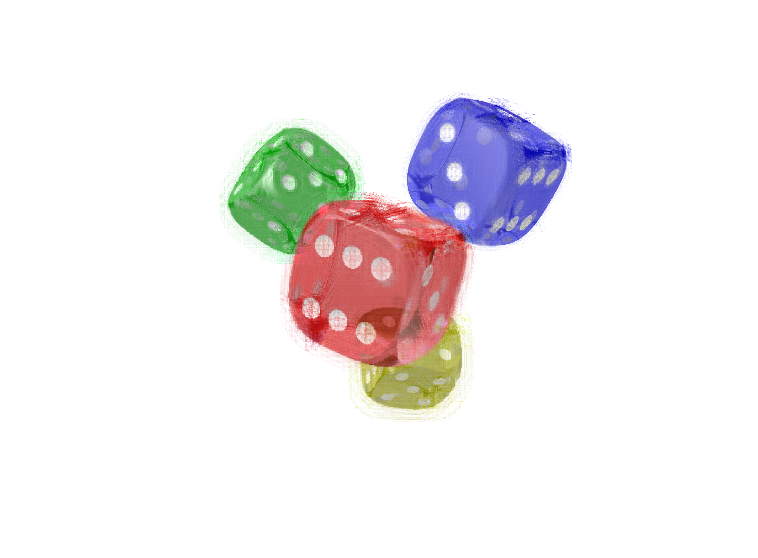
\includegraphics[width=\textwidth]{results/aliasing_fixes/compare_normalization/normalization_r=0_weights=1/central_view_reconstruction2-2.png} 
		\caption{Row-normalization, box radius $0$, $w \equiv 1$.}
		\label{fig:normalization_no_weights}
	\end{subfigure}%
	\\
	\begin{subfigure}[t]{0.45\textwidth}
		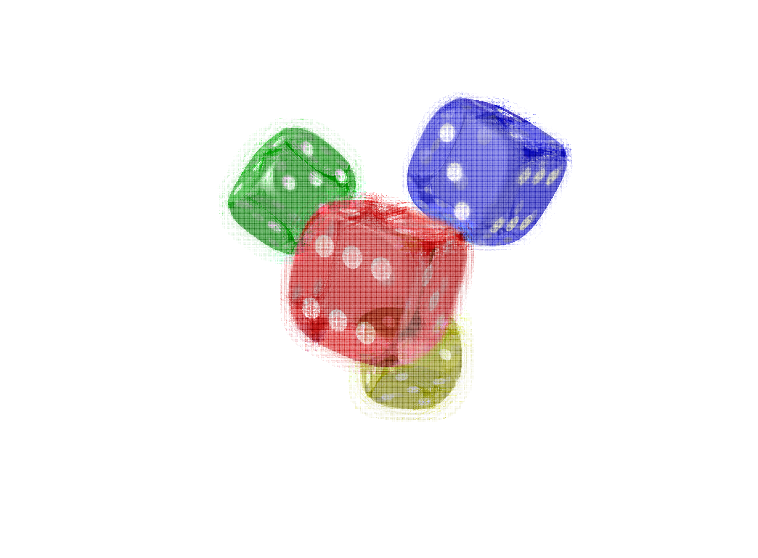
\includegraphics[width=\textwidth]{results/aliasing_fixes/compare_normalization/no_normalization_r=0_weights=gauss/central_view_reconstruction2-2.png} 
		\caption{No normalization, box radius $0$, weights from normal distribution $\mathcal{N}\left(0, 0.3\right)$.}
	\end{subfigure}%
	~
	\begin{subfigure}[t]{0.45\textwidth}
		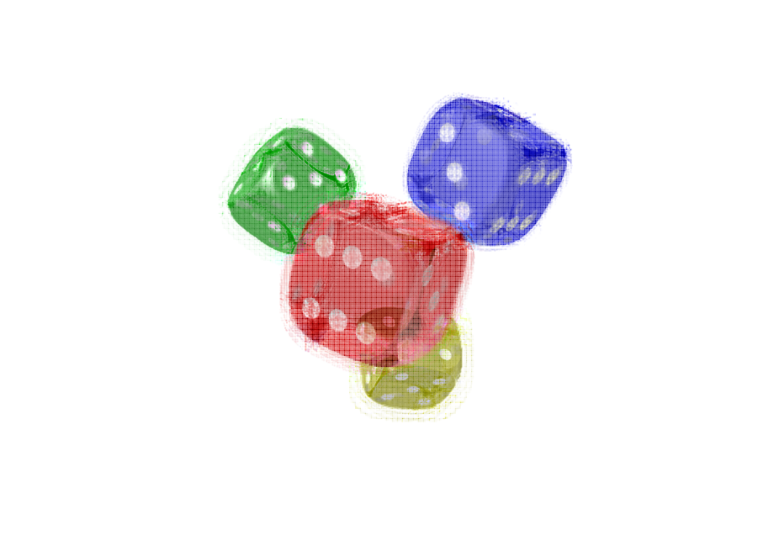
\includegraphics[width=\textwidth]{results/aliasing_fixes/compare_normalization/no_normalization_r=1_weights=gauss/central_view_reconstruction2-2.png} 
		\caption{No normalization, box radius $1$, weights from normal distribution.}
	\end{subfigure}%

	\caption{Reconstructions of the central view $\left(2, 2\right)$ from the $3 \times 3$ dice scene with different parameters.}
	\label{fig:normalization_impact_comparison}
\end{figure}

\subsection{Comparison of the three methods implemented so far}

\begin{enumerate}
	\item	Rays from sensor to layers
		\begin{itemize}
			\item[$-$]	Layer pixels missed by rays	(figure \ref{fig:problem_camera_to_layers})
			\item[$-$]	Artefacts/Aliasing
			\item[$-$]	Sensitive to small parameter changes
			\item[$+$]	No need to adjust/shear the camera images
		\end{itemize}
	\item	Rays from layers to sensor (figure \ref{fig:problem_layers_to_camera})
		\begin{itemize}
			\item[$-$]	Weights only for intersections on sensor 
			\item[$-$]	Artefacts/Aliasing
			\item[$-$]	Sensitive to small parameter changes
			\item[$-$]	Applying box-filter is computationally expensive
			\item[$+$]	Adjustable sampling density of rays
			\item[$+$]	No need to adjust/shear the camera images
		\end{itemize}
	\item	Rays from bottom-most layer, weights for intersection on layers + sensor (figure \ref{fig:intersections_and_weights_overview})
		\begin{itemize}
			\item[$-$]	Normalization of weights along ray cancels out sensor weights
			\item[$-$]	Require rectified images for a common focal plane
			\item[$-$]	Applying box-filter is computationally expensive
			\item[$+$]	Adjustable sampling density of rays
			\item[$+$]	Fewer camera/scene parameters required, less sensitive (if the light field consists of rectified images)
		\end{itemize}
\end{enumerate}

\subsection{Interpolation on the sensor plane}

Instead of rounding the ray intersection points on the sensor to the nearest pixel center and assigning weights to the intersections, we apply linear interpolation to resample the light field. Here are the observations we can make when using the new version of the pipeline:

\begin{itemize}
	\item	Increasing the box radius does not seem to improve the quality of the reconstruction (RMSE)
	\item 	Row normalization is not needed anymore
	\item	Applying weights on the layers according to a gaussian or a tent function introduces line artefacts similar to the ones seen in figure \ref{fig:normalization_impact_comparison} or figure \ref{fig:legotruck_artefacts_r=0}
	\item	Using constant weights $w \equiv 1$ on the layers instead makes the artefacts disappear
	\item 	Increasing the resolution of the layers does not have an impact on the reconstruction quality (RMSE)
\end{itemize}

\begin{figure}
	\centering
	\begin{subfigure}[t]{0.45\textwidth}
		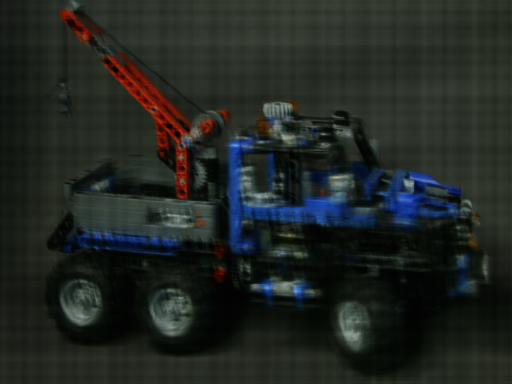
\includegraphics[width=\textwidth]{results/aliasing_fixes/interpolation_on_sensor/legotruck_w=gauss/Reconstruction of view (9, 9).png} 
  		\caption{Reconstruction of view $\left(9, 9\right)$, weights from normal distribution, RMSE: 33.816189.}
	\end{subfigure}%
	~
	\begin{subfigure}[t]{0.45\textwidth}
		\includegraphics[width=\textwidth]{results/aliasing_fixes/interpolation_on_sensor/legotruck_w=gauss/5.png} 
		\caption{Layer 5 (topmost)}
	\end{subfigure}%
	\\
	\begin{subfigure}[t]{0.45\textwidth}
		\includegraphics[width=\textwidth]{results/aliasing_fixes/interpolation_on_sensor/legotruck_w=1/Reconstruction of view (9, 9).png} 
		\caption{Reconstruction of view $\left(9, 9\right)$, $w \equiv 1$, RMSE: 32.503661.}
	\end{subfigure}%
	~
	\begin{subfigure}[t]{0.45\textwidth}
		\includegraphics[width=\textwidth]{results/aliasing_fixes/interpolation_on_sensor/legotruck_w=1/5.png} 
		\caption{Layer 5 (topmost)}
	\end{subfigure}%
	\caption{Comparison of the reconstruction with weights on layers on and off for the legotruck-scene. $9 \times 9$ views, 5 Layers, box-radius 0.}
	\label{fig:comparison_sensor_interpolation_w=1_vs_w=gauss}
\end{figure}

\subsection{Conclusion}

Due to the fact that the intensity of an attenuated light ray is modeled by the Beer-Lambert law, 

\begin{equation}
	I = I_0 e^{-\int_{\mathcal{C}} \! \mu\left(r\right) \, \mathrm{d}r}, 
\end{equation}
and a linear system in the log-domain is needed for the optimization, it is not possible to incorporate interpolation on the attenuation layers. Consider a simple example: Given is a light ray $i$ with intensity $l_i$ passing through an attenuator made of two masks, each having two pixels (see figure~\ref{fig:problem_with_ray_space_interpolation}). The goal is to find attenuation values $a_1$, $a_1^\prime$, $a_2$ and $a_2^\prime$ such that

\begin{equation}
	l_i = \left(\omega_1 a_1 + \left(1 - \omega_1\right) a_1^{\prime}\right) \left(\omega_2 a_2 + \left(1 - \omega_2\right) a_2^{\prime} \right).
\end{equation}
Applying the logarithm gives
\begin{equation}\label{eq:example_ray_interpolation_constraint}
	\bar{l_i} = log\left(l_i\right) = log\left(\omega_1 a_1 + \left(1 - \omega_1\right) a_1^{\prime}\right) + log\left(\omega_2 a_2 + \left(1 - \omega_2\right) a_2^{\prime} \right).
\end{equation}

The problem is that in the log-domain, the constraint~\ref{eq:example_ray_interpolation_constraint} can not be expressed as a linear constraint on the variables $a_1$, $a_1^\prime$, $a_2$ and $a_2^\prime$, such as

\begin{equation}
	\bar{l_i} = P_i x = 
	\begin{bmatrix}
		p_{i1} & p_{i2} & p_{i3} & p_{i4}
	\end{bmatrix}
	\begin{bmatrix}
		a_1 \\ a_1^{\prime} \\ a_2^{\prime} \\ a_2
	\end{bmatrix}.
\end{equation}

\begin{figure}
	\centering
	\includegraphics[height=8cm]{sketches/ray_space_interpolation.pdf}
	\caption{The light ray (red) is attenuated by two layers. The attenuation of the ray at the intersection of a layer is modeled by a weighted sum over the pixel neighbourhood.}
	\label{fig:problem_with_ray_space_interpolation}
\end{figure}

\clearpage
\section{Further improvements for the pipeline}
\subsection{Introduction of the sampling plane}
From now on, the ray density is no longer tied to the resolution of the attenuator or the sensor plane. The introduction of a new and independent plane allows the sampling to be as dense as needed. This new \emph{sampling-plane} has the attributes:

\begin{itemize}
	\item	$z_{sampling}$: It can be placed at any depth. By default, it is set to coincide with the first layer.
	\item	Size: The size of the plane is variable. The default size is the layer size.
	\item	Resolution: The resolution together with the size of the sampling plane define the ray-density.
\end{itemize}

\subsection{Back-Projection and positioning of the layers}
Each layer of the attenuator corresponds to a specific disparity value in the scene. The goal is to optimally place the layers such that all disparities from the light field can be represented by the attenuator. The sensor plane acts as the plane with zero disparity and thus, if the scene has a symmetric disparity range $\left(D_{min} = -D_{max}\right)$, then the sensor plane should be placed at the center of the layer stack. In general, scenes that do not have symmetric disparity range and the sensor plane needs to be shifted inside the  layer stack. 

Back-Projection can be used to make sure that the layers are placed correctly. Once the propagation matrix $P$ has been computed, the back-projection onto the layers can be performed by

\begin{equation} \label{eq:back_projection}
	b = P^T l.
\end{equation}

The vector $b$ holds the result of the back-projection. Equation~\ref{eq:back_projection} corresponds to the sum over all rays passing through a layer pixel. Figure~\ref{fig:comparison_of_two_backprojections} shows two back-projections of a scene with a symmetric disparity range.

\begin{figure}
	\centering
	\begin{subfigure}[t]{0.19\textwidth}
		\includegraphics[width=\textwidth]{results/tarot_back_projection/sensorPlaneZ=-0.5/Back_Projection_layer_1.png} 
	\end{subfigure}%
	~
	\begin{subfigure}[t]{0.19\textwidth}
		\includegraphics[width=\textwidth]{results/tarot_back_projection/sensorPlaneZ=-0.5/Back_Projection_layer_2.png} 
	\end{subfigure}%
	~
	\begin{subfigure}[t]{0.19\textwidth}
		\includegraphics[width=\textwidth]{results/tarot_back_projection/sensorPlaneZ=-0.5/Back_Projection_layer_3.png} 
	\end{subfigure}%
	~
	\begin{subfigure}[t]{0.19\textwidth}
		\includegraphics[width=\textwidth]{results/tarot_back_projection/sensorPlaneZ=-0.5/Back_Projection_layer_4.png} 
	\end{subfigure}%
	~
	\begin{subfigure}[t]{0.19\textwidth}
		\includegraphics[width=\textwidth]{results/tarot_back_projection/sensorPlaneZ=-0.5/Back_Projection_layer_5.png} 
	\end{subfigure}%
	\\\quad
	\begin{subfigure}[t]{0.19\textwidth}
		\includegraphics[width=\textwidth]{results/tarot_back_projection/sensorPlaneZ=-3/Back_Projection_layer_1.png} 
	\end{subfigure}%
	~
	\begin{subfigure}[t]{0.19\textwidth}
		\includegraphics[width=\textwidth]{results/tarot_back_projection/sensorPlaneZ=-3/Back_Projection_layer_2.png} 
	\end{subfigure}%
	~
	\begin{subfigure}[t]{0.19\textwidth}
		\includegraphics[width=\textwidth]{results/tarot_back_projection/sensorPlaneZ=-3/Back_Projection_layer_3.png} 
	\end{subfigure}%
	~
	\begin{subfigure}[t]{0.19\textwidth}
		\includegraphics[width=\textwidth]{results/tarot_back_projection/sensorPlaneZ=-3/Back_Projection_layer_4.png}
	\end{subfigure}%
	~
	\begin{subfigure}[t]{0.19\textwidth}
		\includegraphics[width=\textwidth]{results/tarot_back_projection/sensorPlaneZ=-3/Back_Projection_layer_5.png}
	\end{subfigure}%
	
	\caption{Comparison of two back-projections (top and bottom row) onto five layers (left to right). The first example has the sensor plane at $z_{sensor} = -0.5$, thus zero disparity is mapped onto the middle layer(s). The example below has the sensor plane at $z_{sensor} = -3$. This means that the zero-disparities are mapped onto a layer closer to the observer. The first example is better because it covers the entire depth-range of the scene (the cards in the back are in focus on the first layer and the card in the front is in focus on the 5th layer, not so in the example below).}
	\label{fig:comparison_of_two_backprojections}
\end{figure}

\subsection{Tile-based optimization for attenuation masks}
High resolution light fields can take up a significant amount of space in memory. For example, a light field taken with a Full HD camera from $17\times17$ angles would take up $1920 \cdot 1080 \cdot 17^2 \cdot 3 \cdot 8 / \left(1024^3\right) = 13.3947$ Gigabyte of memory. In addition, the propagation matrix stores information about every pixel in the light field and thus, can take up gigabytes of space depending on the resolution of the attenuation layers. The new approach divides the attenuation layers into tiles. Figure~\ref{fig:sketch_of_tiling_algorithm} shows how the tiles are laid out. Following the notation in figure~\ref{fig:sketch_of_tiling_algorithm},  the inputs for the tiling algorithm are the resolution of the tiles, 
$
r = 
\begin{bmatrix}
	r_x & r_y
\end{bmatrix}
$, and the overlap in horizontal and vertical direction, 
$
o = 
\begin{bmatrix}
	o_x & o_y
\end{bmatrix}
$. The tiles are then laid out in a grid beginning at the top left corner of the layer. The number of tiles needed to cover the plane can be calculated by 

\begin{align*}
	N_x = \left \lceil \dfrac{R_x - o_x}{r_x - o_x} \right \rceil & & N_y = \left \lceil \dfrac{R_y - o_y}{r_y - o_y} \right \rceil.
\end{align*}

The combination of the same tile from each layer forms a new attenuator of smaller size and lower resolution. The optimization is then performed for every tile separately, resulting in a smaller propagation matrix per tile. In the end, the optimized tiles are put together to form the attenuation layers. In general, the borders of the attenuator contain less ray-propagation information and thus, introduce a higher degree of freedom for the optimization. This introduces artefacts that are clearly visible in the reassembled layers as shown in figure~\ref{fig:comparison_tile_overlap_vs_no_overlap}. To solve this issue, the tiles have to overlap. In this case, when reassembling the layers from the tiles, the overlaps need to be blended with a mask: After the optimization, each tile gets multiplied with a mask shown in figure~\ref{fig:quadratic_blending_mask}. The finished layers are then obtained by summing the tiles and dividing by the sum of the blending masks shown in figure~\ref{fig:sum_of_quadratic_blending_masks}.

\begin{figure}
	\centering
	\begin{subfigure}[t]{0.19\textwidth}
		\includegraphics[width=\textwidth]{results/tile_blending/tarot6x6x512x512-512x512x5-sampling=2x_tileRes=200x200_overlap=0/1.png}
	\end{subfigure}%
	~
	\begin{subfigure}[t]{0.19\textwidth}
		\includegraphics[width=\textwidth]{results/tile_blending/tarot6x6x512x512-512x512x5-sampling=2x_tileRes=200x200_overlap=0/2.png}
	\end{subfigure}%
	~
	\begin{subfigure}[t]{0.19\textwidth}
		\includegraphics[width=\textwidth]{results/tile_blending/tarot6x6x512x512-512x512x5-sampling=2x_tileRes=200x200_overlap=0/3.png} 
	\end{subfigure}%
	~
	\begin{subfigure}[t]{0.19\textwidth}
		\includegraphics[width=\textwidth]{results/tile_blending/tarot6x6x512x512-512x512x5-sampling=2x_tileRes=200x200_overlap=0/4.png}
	\end{subfigure}%
	~
	\begin{subfigure}[t]{0.19\textwidth}
		\includegraphics[width=\textwidth]{results/tile_blending/tarot6x6x512x512-512x512x5-sampling=2x_tileRes=200x200_overlap=0/5.png}
	\end{subfigure}%
	\\\quad
	\begin{subfigure}[t]{0.19\textwidth}
		\includegraphics[width=\textwidth]{results/tile_blending/tarot6x6x512x512-512x512x5-sampling=2x_tileRes=200x200_overlap=0.5/1.png} 
	\end{subfigure}%
	~
	\begin{subfigure}[t]{0.19\textwidth}
		\includegraphics[width=\textwidth]{results/tile_blending/tarot6x6x512x512-512x512x5-sampling=2x_tileRes=200x200_overlap=0.5/2.png} 
	\end{subfigure}%
	~
	\begin{subfigure}[t]{0.19\textwidth}
		\includegraphics[width=\textwidth]{results/tile_blending/tarot6x6x512x512-512x512x5-sampling=2x_tileRes=200x200_overlap=0.5/3.png} 
	\end{subfigure}%
	~
	\begin{subfigure}[t]{0.19\textwidth}
		\includegraphics[width=\textwidth]{results/tile_blending/tarot6x6x512x512-512x512x5-sampling=2x_tileRes=200x200_overlap=0.5/4.png}
	\end{subfigure}%
	~
	\begin{subfigure}[t]{0.19\textwidth}
		\includegraphics[width=\textwidth]{results/tile_blending/tarot6x6x512x512-512x512x5-sampling=2x_tileRes=200x200_overlap=0.5/5.png}
	\end{subfigure}%
	
	\caption{Top row: Tiles without overlap. Bottom row: Tiles with 50\% overlap. The layers have a resolution of $512 \times 512$ pixels and the tiles have $200 \times 200$ pixels. The two examples use $3 \times 3$ tiles and $5 \times 5$ tiles respectively.}
	\label{fig:comparison_tile_overlap_vs_no_overlap}
\end{figure}

\begin{figure}
	\centering
	\begin{tabular}[b]{cc}
    	
		\begin{subfigure}[t]{0.6\textwidth}
			\includegraphics[width=\textwidth]{sketches/tiling.pdf}
			\caption{}
			\label{fig:sketch_of_tiling_algorithm}
		\end{subfigure}%
		&
		\begin{tabular}[b]{c}			
			
			\begin{subfigure}[t]{0.25\textwidth}
				\includegraphics[width=\textwidth]{results/tile_blending/quadratic_tile_blending_mask.png}
				\caption{}
				\label{fig:quadratic_blending_mask}
			\end{subfigure}%
			\\
			\begin{subfigure}[t]{0.25\textwidth}
				\includegraphics[width=\textwidth]{results/tile_blending/tarot6x6x512x512-512x512x5-sampling=2x_tileRes=200x200_overlap=0.5/blendingMaskSum.png}
				\caption{}
				\label{fig:sum_of_quadratic_blending_masks}
			\end{subfigure}%
			
		\end{tabular}
	\end{tabular}
	
	\caption{A plane of size $R_x \times R_y$ pixels is covered by tiles of size $r_x \times r_y$ pixels. The tiles overlap by $o_x$ pixels in horizontal direction and by $o_y$ pixels in vertical direction. A quadratic mask (b) is used to blend the overlaps of the tiles. The sum of the masks is shown in (c).}
	\label{fig:blending_mask_for_tiles}
\end{figure}

\begin{figure}
	\centering
	\begin{subfigure}[t]{0.3\textwidth}
		\includegraphics[width=\textwidth]{results/tile_blending/tarot6x6x512x512-512x512x5-sampling=2x_tileRes=200x200_overlap=0.5/Reconstruction_of_view_(1,1).png}
		\caption{(1,1)}
	\end{subfigure}%
	~
	\begin{subfigure}[t]{0.3\textwidth}
		\includegraphics[width=\textwidth]{results/tile_blending/tarot6x6x512x512-512x512x5-sampling=2x_tileRes=200x200_overlap=0.5/Reconstruction_of_view_(1,3).png}
		\caption{(1,3)}
	\end{subfigure}%
	~
	\begin{subfigure}[t]{0.3\textwidth}
		\includegraphics[width=\textwidth]{results/tile_blending/tarot6x6x512x512-512x512x5-sampling=2x_tileRes=200x200_overlap=0.5/Reconstruction_of_view_(1,6).png} 
		\caption{(1,6)}
	\end{subfigure}%
	\\
	\begin{subfigure}[t]{0.3\textwidth}
		\includegraphics[width=\textwidth]{results/tile_blending/tarot6x6x512x512-512x512x5-sampling=2x_tileRes=200x200_overlap=0.5/Reconstruction_of_view_(3,1).png}
		\caption{(3,1)}
	\end{subfigure}%
	~
	\begin{subfigure}[t]{0.3\textwidth}
		\includegraphics[width=\textwidth]{results/tile_blending/tarot6x6x512x512-512x512x5-sampling=2x_tileRes=200x200_overlap=0.5/Reconstruction_of_view_(3,3).png}
		\caption{(3,3)}
	\end{subfigure}%
	~
	\begin{subfigure}[t]{0.3\textwidth}
		\includegraphics[width=\textwidth]{results/tile_blending/tarot6x6x512x512-512x512x5-sampling=2x_tileRes=200x200_overlap=0.5/Reconstruction_of_view_(3,6).png} 
		\caption{(3,6)}
	\end{subfigure}%
	\\
	\begin{subfigure}[t]{0.3\textwidth}
		\includegraphics[width=\textwidth]{results/tile_blending/tarot6x6x512x512-512x512x5-sampling=2x_tileRes=200x200_overlap=0.5/Reconstruction_of_view_(6,1).png} 
		\caption{(6,1)}
	\end{subfigure}%
	~
	\begin{subfigure}[t]{0.3\textwidth}
		\includegraphics[width=\textwidth]{results/tile_blending/tarot6x6x512x512-512x512x5-sampling=2x_tileRes=200x200_overlap=0.5/Reconstruction_of_view_(6,3).png} 
		\caption{(6,3)}
	\end{subfigure}%
	~
	\begin{subfigure}[t]{0.3\textwidth}
		\includegraphics[width=\textwidth]{results/tile_blending/tarot6x6x512x512-512x512x5-sampling=2x_tileRes=200x200_overlap=0.5/Reconstruction_of_view_(6,6).png}
		\caption{(6,6)}
	\end{subfigure}%
	
	\caption{Reconstructed views from the attenuation layers created with tiles shown in figure~\ref{fig:comparison_tile_overlap_vs_no_overlap}.}
	\label{fig:Reconstructions_from_tiled_attenuator}
\end{figure}

\begin{figure}
	\centering
	\begin{subfigure}[t]{0.3\textwidth}
		\includegraphics[width=\textwidth]{results/tile_blending/tarot6x6x512x512-512x512x5-sampling=2x_tileRes=200x200_overlap=0.5/MSE_for_view_(1,1).png}
		\caption{(1,1), 38.874372}
	\end{subfigure}%
	~
	\begin{subfigure}[t]{0.3\textwidth}
		\includegraphics[width=\textwidth]{results/tile_blending/tarot6x6x512x512-512x512x5-sampling=2x_tileRes=200x200_overlap=0.5/MSE_for_view_(1,3).png}
		\caption{(1,3), 31.726001}
	\end{subfigure}%
	~
	\begin{subfigure}[t]{0.3\textwidth}
		\includegraphics[width=\textwidth]{results/tile_blending/tarot6x6x512x512-512x512x5-sampling=2x_tileRes=200x200_overlap=0.5/MSE_for_view_(1,6).png} 
		\caption{(1,6), 40.818872}
	\end{subfigure}%
	\\
	\begin{subfigure}[t]{0.3\textwidth}
		\includegraphics[width=\textwidth]{results/tile_blending/tarot6x6x512x512-512x512x5-sampling=2x_tileRes=200x200_overlap=0.5/MSE_for_view_(3,1).png}
		\caption{(3,1), 34.764987}
	\end{subfigure}%
	~
	\begin{subfigure}[t]{0.3\textwidth}
		\includegraphics[width=\textwidth]{results/tile_blending/tarot6x6x512x512-512x512x5-sampling=2x_tileRes=200x200_overlap=0.5/MSE_for_view_(3,3).png}
		\caption{(3,3), 29.083222}
	\end{subfigure}%
	~
	\begin{subfigure}[t]{0.3\textwidth}
		\includegraphics[width=\textwidth]{results/tile_blending/tarot6x6x512x512-512x512x5-sampling=2x_tileRes=200x200_overlap=0.5/MSE_for_view_(3,6).png} 
		\caption{(3,6), 33.866169}
	\end{subfigure}%
	\\
	\begin{subfigure}[t]{0.3\textwidth}
		\includegraphics[width=\textwidth]{results/tile_blending/tarot6x6x512x512-512x512x5-sampling=2x_tileRes=200x200_overlap=0.5/MSE_for_view_(6,1).png} 
		\caption{(6,1), 46.360238}
	\end{subfigure}%
	~
	\begin{subfigure}[t]{0.3\textwidth}
		\includegraphics[width=\textwidth]{results/tile_blending/tarot6x6x512x512-512x512x5-sampling=2x_tileRes=200x200_overlap=0.5/MSE_for_view_(6,3).png} 
		\caption{(6,3), 37.760786}
	\end{subfigure}%
	~
	\begin{subfigure}[t]{0.3\textwidth}
		\includegraphics[width=\textwidth]{results/tile_blending/tarot6x6x512x512-512x512x5-sampling=2x_tileRes=200x200_overlap=0.5/MSE_for_view_(6,6).png}
		\caption{(6,6), 42.153688}
	\end{subfigure}%
	
	\caption{Mean square error (MSE) images for the reconstructed views in figure~\ref{fig:Reconstructions_from_tiled_attenuator}. The root mean square error (RMSE) is written besides the angular coordinate.}
	\label{fig:MSE_for_reconstructions_from_tiled_attenuator}
\end{figure}


\begin{figure}
	\centering
	\begin{subfigure}[t]{0.31\textwidth}
		\includegraphics[width=\textwidth]{results/tiles_legotruck_6x6x480x640_480x640x5_tiling_4x6x200x200_overlap_0.5/1.png}
		\caption{Layer 1}
	\end{subfigure}%
	~
	\begin{subfigure}[t]{0.31\textwidth}
		\includegraphics[width=\textwidth]{results/tiles_legotruck_6x6x480x640_480x640x5_tiling_4x6x200x200_overlap_0.5/2.png}
		\caption{Layer 2}
	\end{subfigure}%
	~
	\begin{subfigure}[t]{0.31\textwidth}
		\includegraphics[width=\textwidth]{results/tiles_legotruck_6x6x480x640_480x640x5_tiling_4x6x200x200_overlap_0.5/3.png}
		\caption{Layer 3}
	\end{subfigure}%
	\\
	\begin{subfigure}[t]{0.31\textwidth}
		\includegraphics[width=\textwidth]{results/tiles_legotruck_6x6x480x640_480x640x5_tiling_4x6x200x200_overlap_0.5/4.png}
		\caption{Layer 4}
	\end{subfigure}%
	~
	\begin{subfigure}[t]{0.31\textwidth}
		\includegraphics[width=\textwidth]{results/tiles_legotruck_6x6x480x640_480x640x5_tiling_4x6x200x200_overlap_0.5/5.png}
		\caption{Layer 1}
	\end{subfigure}%
	\\
	\begin{subfigure}[t]{0.31\textwidth}
		\includegraphics[width=\textwidth]{results/tiles_legotruck_6x6x480x640_480x640x5_tiling_4x6x200x200_overlap_0.5/Reconstruction_of_view_(1,1).png}
		\caption{(1,1)}
	\end{subfigure}%
	~
	\begin{subfigure}[t]{0.31\textwidth}
		\includegraphics[width=\textwidth]{results/tiles_legotruck_6x6x480x640_480x640x5_tiling_4x6x200x200_overlap_0.5/Reconstruction_of_view_(1,3).png}
		\caption{(1,3)}
	\end{subfigure}%
	~
	\begin{subfigure}[t]{0.31\textwidth}
		\includegraphics[width=\textwidth]{results/tiles_legotruck_6x6x480x640_480x640x5_tiling_4x6x200x200_overlap_0.5/Reconstruction_of_view_(1,6).png}
		\caption{(1,6)}
	\end{subfigure}%
	\\
	\begin{subfigure}[t]{0.31\textwidth}
		\includegraphics[width=\textwidth]{results/tiles_legotruck_6x6x480x640_480x640x5_tiling_4x6x200x200_overlap_0.5/Reconstruction_of_view_(3,1).png}
		\caption{(3,1)}
	\end{subfigure}%
	~
	\begin{subfigure}[t]{0.31\textwidth}
		\includegraphics[width=\textwidth]{results/tiles_legotruck_6x6x480x640_480x640x5_tiling_4x6x200x200_overlap_0.5/Reconstruction_of_view_(3,3).png}
		\caption{(3,3)}
	\end{subfigure}%
	~
	\begin{subfigure}[t]{0.31\textwidth}
		\includegraphics[width=\textwidth]{results/tiles_legotruck_6x6x480x640_480x640x5_tiling_4x6x200x200_overlap_0.5/Reconstruction_of_view_(3,6).png}
		\caption{(3,6)}
	\end{subfigure}%
	\\
	\begin{subfigure}[t]{0.31\textwidth}
		\includegraphics[width=\textwidth]{results/tiles_legotruck_6x6x480x640_480x640x5_tiling_4x6x200x200_overlap_0.5/Reconstruction_of_view_(6,1).png}
		\caption{(6,1)}
	\end{subfigure}%
	~
	\begin{subfigure}[t]{0.31\textwidth}
		\includegraphics[width=\textwidth]{results/tiles_legotruck_6x6x480x640_480x640x5_tiling_4x6x200x200_overlap_0.5/Reconstruction_of_view_(6,3).png}
		\caption{(6,3)}
	\end{subfigure}%
	~
	\begin{subfigure}[t]{0.31\textwidth}
		\includegraphics[width=\textwidth]{results/tiles_legotruck_6x6x480x640_480x640x5_tiling_4x6x200x200_overlap_0.5/Reconstruction_of_view_(6,6).png}
		\caption{(6,6)}
	\end{subfigure}%
	
	\caption{The legotruck scene, produced by 5 attenuation layers (a) to (e) using $4 \times 6$ tiles of size $200 \times 200$ with an overlap of 50\%. Below are the reconstructions of the views (f) to (n) from the $6 \times 6$ camera grid (every other left out).}
	\label{fig:Legotruck_scene_layers and_reconstructions_using_tiles}
\end{figure}


\begin{figure}
	\centering
	\begin{subfigure}[t]{0.31\textwidth}
		\includegraphics[width=\textwidth]{results/tiles_legotruck_6x6x480x640_480x640x5_tiling_4x6x200x200_overlap_0.5/MSE_for_view_(1,1).png}
		\caption{(1,1), 19.964930}
	\end{subfigure}%
	~
	\begin{subfigure}[t]{0.31\textwidth}
		\includegraphics[width=\textwidth]{results/tiles_legotruck_6x6x480x640_480x640x5_tiling_4x6x200x200_overlap_0.5/MSE_for_view_(1,3).png}
		\caption{(1,3), 17.466928}
	\end{subfigure}%
	~
	\begin{subfigure}[t]{0.31\textwidth}
		\includegraphics[width=\textwidth]{results/tiles_legotruck_6x6x480x640_480x640x5_tiling_4x6x200x200_overlap_0.5/MSE_for_view_(1,6).png}
		\caption{(1,6), 21.811898}
	\end{subfigure}%
	\\
	\begin{subfigure}[t]{0.31\textwidth}
		\includegraphics[width=\textwidth]{results/tiles_legotruck_6x6x480x640_480x640x5_tiling_4x6x200x200_overlap_0.5/MSE_for_view_(3,1).png}
		\caption{(3,1), 16.095934}
	\end{subfigure}%
	~
	\begin{subfigure}[t]{0.31\textwidth}
		\includegraphics[width=\textwidth]{results/tiles_legotruck_6x6x480x640_480x640x5_tiling_4x6x200x200_overlap_0.5/MSE_for_view_(3,3).png}
		\caption{(3,3), 13.945447}
	\end{subfigure}%
	~
	\begin{subfigure}[t]{0.31\textwidth}
		\includegraphics[width=\textwidth]{results/tiles_legotruck_6x6x480x640_480x640x5_tiling_4x6x200x200_overlap_0.5/MSE_for_view_(3,6).png}
		\caption{(3,6), 17.585800}
	\end{subfigure}%
	\\
	\begin{subfigure}[t]{0.31\textwidth}
		\includegraphics[width=\textwidth]{results/tiles_legotruck_6x6x480x640_480x640x5_tiling_4x6x200x200_overlap_0.5/MSE_for_view_(6,1).png}
		\caption{(6,1), 20.407914}
	\end{subfigure}%
	~
	\begin{subfigure}[t]{0.31\textwidth}
		\includegraphics[width=\textwidth]{results/tiles_legotruck_6x6x480x640_480x640x5_tiling_4x6x200x200_overlap_0.5/MSE_for_view_(6,3).png}
		\caption{(6,3), 17.096632}
	\end{subfigure}%
	~
	\begin{subfigure}[t]{0.31\textwidth}
		\includegraphics[width=\textwidth]{results/tiles_legotruck_6x6x480x640_480x640x5_tiling_4x6x200x200_overlap_0.5/MSE_for_view_(6,6).png}
		\caption{(6,6), 20.560457}
	\end{subfigure}%
	
	\caption{Mean square error (MSE) images for the reconstructed views in figure~\ref{fig:Legotruck_scene_layers and_reconstructions_using_tiles}. The root mean square error (RMSE) is written besides the angular coordinate.}
	\label{fig:MSE_for_legotruck_scene_reconstruction_with_tiles}
\end{figure}

\clearpage
\bibliographystyle{alpha}
\bibliography{lit}

\end{document}

